\documentclass[12pt]{tcc} 
\usepackage[brazil]{babel} 
\usepackage[T1]{fontenc}
\usepackage{datetime2}
\DTMsetdatestyle{ddmmyyyy}
\usepackage[acronym, nomain]{glossaries}
\usepackage{makecell}

\newacronym{ARIMA}{ARIMA}{AutoRegressive Integrated Moving Average}
\newacronym{ARMA}{ARMA}{AutoRegressive Moving Average}
\newacronym{PPA}{PPA}{Plano Plurianual}
\newacronym{LDO}{LDO}{Lei de Diretrizes Orçamentárias}
\newacronym{LOA}{LOA}{Lei Orçamentária Anual}
\newacronym{MMS}{MMS}{Média Móvel Simples}
\newacronym{SOF}{SOF}{Secretaria de Orçamento Federal}
\newacronym{SETTRAN}{SETTRAN}{Secretaria Municipal de Trânsito e Transportes}
\newacronym{SMTR}{SMTR}{Secretaria Municipal de Trânsito do Rio de Janeiro}
\newacronym{SMAPE}{SMAPE}{Symmetric Mean Absolute Percentage Error}
\newacronym{MSE}{MSE}{Mean Squared Error}
\newacronym{R2}{$R^2$}{R-Squared}
\newacronym{ML}{ML}{Aprendizado de Máquina}

\newacronym{MLP}{MLP}{Multi Layer Perceptron}
\newacronym{KNN}{KNN}{K-Nearest Neighbour}

\usepackage{graphicx}
\usepackage{comment}
\usepackage{soul}

\usepackage{amsmath}
\usepackage{amssymb}
\usepackage{algorithm}
\usepackage{algpseudocode}

\graphicspath{{./figures/}}

\newcommand\dtitle{Previsão de Receitas de Multas de Trânsito do Município do Rio de Janeiro}
\newcommand\dauthor{Carlos Henrique de Oliveira Pereira}
\newcommand\dadvisor{Eduardo Soares Ogasawara, D.Sc.\\Boris Marinho Ramos Silva Araujo}

\makeglossaries

\newacronym{TCC}{TCC}{Trabalho de Conclusão de Curso}

\begin{document}
\pagenumbering{gobble}
\pagenumbering{roman}

\dcover

\dcoverback

\dlibrary{ficha.pdf}

\ddedicatory{
	\raggedleft \normalsize 
Dedico este trabalho:

\vspace{0.5cm}

\noindent Aos meus familiares, pelo apoio incondicional e pela paciência nos momentos desafiadores, que são pilares fundamentais ao longo da minha trajetória.

\vspace{0.5cm}

\noindent Aos meus professores e orientadores, pela transmissão de conhecimento, pelo incentivo constante e pela orientação que possibilita a realização desta conquista.

\vspace{0.5cm}

\noindent Aos meus amigos, pelas risadas que trazem leveza, pelas palavras de incentivo nos momentos de dúvida e pela companhia presente nos instantes de descontração, essenciais para manter o equilíbrio e a motivação.

\vspace{1cm} 

\noindent Esta conquista também é fruto do apoio de cada um de vocês.

\vspace{2cm} 

\hfill Com gratidão, \\
\hfill Carlos Henrique de Oliveira Pereira.
}

\dacknowledgment{
	Agradece-se à CAPES, CNPq e FAPERJ pelo financiamento parcial desta pesquisa.
}

\dresumo{
O financiamento de investimentos realizados por órgãos de mobilidade urbana é crítico, pois, mesmo gerando impactos positivos com melhorias em sinalizações e estruturas viárias, pode prejudicar a instituição quando feito sem planejamento adequado. Parte das receitas dessas instituições provém de multas de trânsito, o que torna relevante o estudo de técnicas de previsão de receitas futuras para um planejamento mais preciso. Neste estudo, são realizados experimentos de previsão em séries temporais com alguns modelos de aprendizado de máquina, disponibilizados na biblioteca TSPrediT. O objetivo principal é investigar o desempenho desses modelos na previsão de receitas do município do Rio de Janeiro, com base nas métricas de erro $R^2$, SMAPE e MSE. Os modelos de aprendizado de máquina mostraram-se relevantes na previsão de receitas, tendo como destaque o modelo MLP que obteve um valor de $R^2$ de 60.26\%. 
}{Séries temporais; Agregação temporal; Aprendizado de Máquina; Previsão de receitas; Multas de trânsito.}

\dabstract{
Financing investments carried out by urban mobility agencies is critical because, despite generating positive impacts through improvements in signaling and road infrastructure, it can jeopardize the institution when conducted without proper planning. Since a portion of these institutions' revenue stems from traffic fines, the study of techniques for forecasting future revenue becomes essential for more accurate planning. In this study, time series forecasting experiments are performed using various machine learning models available in the TSPrediT library. The primary objective is to investigate the performance of these models in forecasting revenue for the municipality of Rio de Janeiro, based on the error metrics $R^2$, SMAPE, and MSE. Machine learning models proved to be relevant for revenue forecasting, with the MLP model standing out by achieving an $R^2$ value of 60.26\%.
}{Time series; Temporal aggregation; Machine Learning; Revenue forecasting; Traffic fines.}

\dtables

\pagenumbering{arabic}
\justifying

\chapter{Introdução}
\label{sec:introducao}

O modelo orçamentário brasileiro vigente foi consolidado com a Constituição Federal de 1988 e tem como objetivo o planejamento e o gerenciamento das finanças públicas do país \citep{deputados_constituicao_2025}. Ele é composto por três elementos-base: o \gls{PPA}, a \gls{LDO} e a \gls{LOA}. O \gls{PPA} estabelece as diretrizes, os objetivos e as metas de médio prazo da administração pública, orientando, de forma conjunta, a \gls{LDO} e a \gls{LOA}. A \gls{LDO} define os parâmetros necessários para a alocação de recursos no orçamento anual, assegurando a realização das metas e dos objetivos contemplados no \gls{PPA}. A \gls{LOA} permite estimar receitas e fixar despesas, viabilizando análises sobre a origem e a destinação dos recursos públicos. Dessa forma, a legislação brasileira orienta os órgãos públicos a cumprirem as metas e os objetivos estabelecidos.

O orçamento é um documento central da política que viabiliza a execução de programas governamentais destinados a beneficiar a sociedade e promover melhorias no país \citep{speeden_fatores_2019}. O município é o ente subnacional mais capacitado para solucionar problemas locais, pois possui o conhecimento mais preciso sobre suas prioridades e os impactos das demandas sociais de sua população \citep{louzano_causalidade_2019}. No contexto da mobilidade urbana, o orçamento é planejado com foco em melhorias nas vias públicas, na sinalização viária, na implementação de novas rotas de trânsito, no subsídio tarifário ao transporte público, entre outras intervenções voltadas à circulação, à segurança viária e à promoção da mobilidade urbana. A arrecadação de multas de trânsito é uma fonte de receita substancial para o setor, somando mais de 304 milhões no Rio de Janeiro em 2024, de acordo com dados da prefeitura \citep{limaNetoRJMultasArrecadacaoGlobo}.

Um planejamento orçamentário adequado é essencial para viabilizar o financiamento dos serviços e dos programas públicos \citep{nascimento_fatores_2022}. A maior precisão na previsão das receitas públicas traz benefícios para a gestão da mobilidade urbana, pois contribui para a estabilidade do financiamento e reduz o risco de descontinuidade das ações planejadas \citep{da2017orccamento}. Previsões mais precisas de receita favorecem a execução orçamentária e aumentam a estabilidade no financiamento das despesas previstas na \gls{LOA}.

Este trabalho experimenta e avalia a possibilidade de utilização de um modelo de aprendizado de máquina capaz de prever receitas de multas de trânsito em uma janela de um ano, aplicando agregação temporal para reduzir os ruídos e melhorar o desempenho preditivo dos modelos na previsão de receitas de multas de trânsito do município do Rio de Janeiro. O estudo considera horizontes de previsão de um ano, em função da aplicabilidade prática no contexto do planejamento orçamentário municipal. Assim, os experimentos são executados com a transformação da série temporal. A série apresenta mudanças abruptas de comportamento no período entre 2020 e 2022, possivelmente explicadas por alterações legislativas durante a pandemia de COVID-19, porém não se aplicam técnicas de modelagem de rupturas estruturais devido à baixa frequência do evento e à dificuldade de parametrização adequada.

Quanto às métricas de avaliação dos resultados obtidos, observa-se que a série temporal com suavização de $k=1$, ou seja, a série sem qualquer transformação, apresenta valor de \gls{R2} mais elevado em comparação com as demais séries. Também se verifica que, à medida que o grau de suavização aumenta, o valor do \gls{SMAPE} diminui. Não se obtêm conclusões quanto à métrica \gls{MSE}.

Embora diversas pesquisas apresentem bons resultados ao prever receitas públicas com modelos \gls{ARIMA}, o conjunto de dados utilizado apresenta uma variação atípica que pode impactar negativamente o desempenho do modelo. Apesar da quebra estrutural da série, é possível que existam métodos mais eficazes para essa tarefa. Modelos mais sofisticados, como Redes Neurais, Long Short-Term Memory (LSTM) e k-Nearest Neighbors(KNN), podem ser vantajosos. Portanto, recomenda-se o estudo de novos métodos para previsão de receitas, especificamente para esta série temporal.

Além da introdução, este trabalho está organizado em mais cinco capítulos. O Capítulo \ref{sec:fund_teorica} apresenta a fundamentação teórica. O Capítulo \ref{sec:trabalhos_relacionados} apresenta os trabalhos relacionados. O Capítulo \ref{sec:metodologia} descreve o método. No Capítulo \ref{sec:resultados}, são mostrados os resultados. E, por fim, no Capítulo \ref{sec:conclusao} é apresentada a conclusão.

\chapter{Fundamentação teórica}
\label{sec:background}
\label{sec:fund_teorica}

Este capítulo apresenta os conceitos essenciais para o entendimento deste trabalho. A Seção \ref{sec:series_temporais} resume os elementos fundamentais de uma série temporal. A Seção \ref{sec:indicadores_desempenho} descreve os indicadores de desempenho, importantes para a compreensão e interpretação dos resultados preliminares. A Seção \ref{sec:arima} explica o \gls{ARIMA}, um modelo de previsão amplamente utilizado em séries temporais. A Seção \ref{eq:media_movel} resume a \gls{MMS}, uma técnica utilizada para suavizar séries temporais. A Seção \ref{sec:agregacao_temporal} apresenta a agregação temporal, uma técnica que transforma a série a partir do agrupamento de observações próximas.

\section{Séries Temporais}
\label{sec:series_temporais}

Uma série temporal é uma sequência $(x_1, x_2, \dots, x_n)$ separada por um intervalo fixo de tempo (por exemplo, segundos, horas ou dias). Esses dados podem ser agregados em intervalos maiores, como quinzenas, semanas ou trimestres \citep{gujarati_basic_2003}. As séries temporais podem ser univariadas, quando há observações de apenas uma variável, ou multivariadas, quando há observações de duas ou mais variáveis. No caso multivariado, podem ser exploradas relações entre as variáveis para aumentar o desempenho do modelo \citep{silvestrini2008temporal}. 

É possível decompor uma série temporal em três componentes: tendência, sazonalidade e resíduo. Cada componente contém informações relevantes sobre o comportamento da série, auxiliando em análises mais precisas e na identificação de padrões \citep{ogasawara_event_2025}.

A tendência é a componente que indica o movimento da série temporal ao longo do tempo. Ela revela se a série é crescente, decrescente ou estável em determinado intervalo \citep{ogasawara_event_2025}. Um exemplo de tendência crescente é o uso de inteligências artificiais generativas nos últimos anos.

A sazonalidade representa padrões que se repetem em intervalos regulares, como dias, meses ou anos. Esses padrões são frequentemente observados em setores de vendas, por exemplo. O aumento da demanda por presentes no período natalino é um exemplo característico dessa componente \citep{ogasawara_event_2025, zellner_seasonal_1978}.

O resíduo refere-se ao que permanece após a remoção da tendência e da sazonalidade. Trata-se das variações não explicadas pelos demais componentes, mas que ainda compõem parte relevante das observações. A decomposição auxilia na análise e na compreensão da estrutura da série temporal, assegurando que as variações desordenadas permaneçam apenas nos resíduos \citep{ogasawara_event_2025}.

A série é dita estacionária quando sua tendência e sazonalidade são nulas. Isso significa que seus valores não estão correlacionados com o tempo e que sua média e variância são constantes. Esse comportamento também pode ser denominado ruído branco \citep{hyndman_forecasting_2018,sato_gerenciamento_2013}.

Como o modelo \gls{ARIMA} requer estacionaridade, procedimentos como diferenciação e suavização são frequentemente aplicados para eliminar a tendência e a sazonalidade, estabilizando a média e a variância da série \citep{sato_gerenciamento_2013}.

\begin{figure}[!ht]
    \centering
    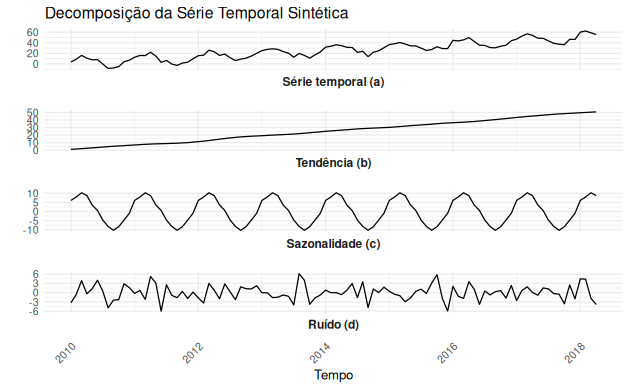
\includegraphics[width=0.9\linewidth]{decomposicao_exemplo2.png}
    \caption{Exemplo de decomposição}
    \label{fig:Exempo de um série temporal decomposta}
\end{figure}

\begin{figure}[!ht]
	\centering
	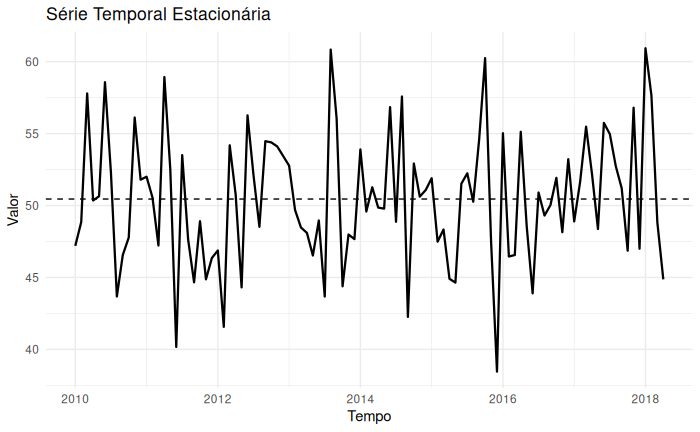
\includegraphics[width=0.6\textwidth]{figures/serie_temporal_estacionaria_exemplo1.png}
	\caption{Exemplo de série temporal estacionária. A linha tracejada indica a média da série temporal.}
	\label{fig:exemplo}
\end{figure}

\section{Indicadores de desempenho}
\label{sec:indicadores_desempenho}

Em todo modelo preditivo, é necessário analisar seu desempenho e compará-lo com outros modelos para obter resultados confiáveis \citep{hyndman_forecasting_2018}. Há diversos métodos para avaliar o desempenho desses modelos. Neste trabalho, utilizam-se três métricas: \acrshort{MSE}, \acrshort{SMAPE} e o Coeficiente de Determinação (\acrshort{R2}).

Para as equações a seguir, $n$ é o número de previsões, $y_t$ é a observação original, $\hat{y}_t$ é a previsão da série e $t$ representa o tempo.

Representado pela fórmula \ref{eq:smape}, o \acrfull{SMAPE} é uma métrica baseada na porcentagem do erro. Essa métrica é útil para valores com grande variação de escala. Seu resultado pode variar de \( 0 \), quando não há erro, até \( +\infty \), indicando o pior caso nas previsões \citep{ogasawara_event_2025}.

O \acrfull{MSE} é uma métrica calculada na mesma escala dos dados. Como mostrado na fórmula \ref{eq:mse}, é sensível a outliers devido à operação de elevação ao quadrado \citep{chen_new_2017}. Pode variar de \( 0 \), em caso de erro nulo, até \( +\infty \), sendo que valores mais altos indicam pior desempenho.

Definido pela fórmula \ref{eq:rsquared}, o \acrfull{R2} é uma métrica que mede a proporção da variabilidade da variável dependente explicada pelo modelo \citep{chicco_coefficient_2021}. Em outras palavras, avalia o grau de ajuste entre os dados previstos e os dados observados. Pode variar de \( -\infty \) a \( 1 \), sendo que valores próximos de \( 1 \) indicam bom ajuste. Quando ${R^2} = 1$, o modelo representa perfeitamente os dados reais. Valores positivos indicam ajuste satisfatório, enquanto valores negativos indicam ajuste inadequado.

\begin{equation}
\text{SMAPE} = \frac{100}{n} \sum_{t=1}^{n} \frac{\left| y_t - \hat{y}_t \right|}{(\left| y_t \right| + \left| \hat{y}_t \right|)/2}
\label{eq:smape}
\end{equation}

\begin{equation}
\text{MSE} = \frac{1}{n} \sum_{t=1}^{n} (\hat{y}_t - y_t)^2
\label{eq:mse}
\end{equation}

\begin{equation}
\boldsymbol{R^2} = 1 - \frac{\sum_{t=1}^{n} (\hat{y}_t - y_t)^2}{\sum_{t=1}^{n} (\bar{y} - y_t)^2}
\label{eq:rsquared}
\end{equation}

Enquanto o \gls{MSE} mede o desempenho de forma relativa e dependente da escala, penalizando fortemente outliers, o \gls{SMAPE}, por ser percentual, apresenta maior robustez frente a variações de escala, tornando-se sensível em séries com alta dispersão. A análise combinada de \gls{SMAPE}, \gls{MSE} e \gls{R2} permite avaliar a acurácia, a variabilidade e o grau de explicação da previsão, sendo necessária para a interpretação crítica do desempenho preditivo \citep{hyndman_forecasting_2018}.

\section{Critério AIC}
\label{sec:aic}

O Critério de Informação de Akaike, abreviado como AIC, é uma métrica estatística utilizada para selecionar modelos que tentam equilibrar a simplicidade e a explicabilidade dos dados. Proposto por Hirotugu Akaike em 1974, o critério baseia-se na teoria da informação e na busca pela minimização da perda de informação ao representar uma série real por meio de uma equação matemática. A base teórica do AIC é a Divergência de Kullback-Leibler, que mede a diferença entre o modelo candidato proposto e o modelo verdadeiro. O AIC funciona como uma estimativa dessa diferença; portanto, quanto menor o valor do AIC, mais próximo o modelo candidato está de representar a realidade sem perda excessiva de informação \citep{vrieze2012model}.

Na equação \ref{eq:aic}, o $L$ representa a máxima verossimilhança do modelo, indicando o quão bem o modelo explica os dados observados, e $k$ é o número de parâmetros estimados. O termo $2k$ atua como uma penalidade: quanto mais complexo o modelo, maior será o valor do AIC, exceto se esse aumento de complexidade resultar em um ganho significativo de ajuste.

\begin{equation}
\text{AIC} = -2\ln(L) + 2k
\label{eq:aic}
\end{equation}

\section{Arima}
\label{sec:arima}

Denominado extensivamente como \acrlong{ARIMA}, o \gls{ARIMA} é um modelo autorregressivo de previsão amplamente utilizado desde sua criação, em 1970, por George Box e Gwilym Jenkins. Seu funcionamento baseia-se na identificação de padrões nos dados para a obtenção de operadores que, combinados, formam uma equação linear representativa da série temporal \citep{BoxJenkins1970}. No modelo \textit{ARIMA}($p$, $d$, $q$), $p$ representa o grau da parte autorregressiva, $d$ o grau da diferenciação e $q$ o grau da parte de média móvel \citep{sato_gerenciamento_2013, hyndman_automatic_2008}. Dependendo dos valores desses parâmetros, o modelo apresenta configurações específicas. Um exemplo é o ARIMA(0, 1, 0), conhecido como \textit{Random Walk}. O \textit{Auto ARIMA} é uma função que determina automaticamente os valores de $p$, $d$ e $q$ com base no melhor valor do AIC, critério utilizado para avaliar a qualidade de modelos estatísticos \citep{hyndman_automatic_2008}.

Esse modelo é utilizado preferencialmente com séries estacionárias. Quando a série não é estacionária, aplica-se a diferenciação, que consiste no cálculo da diferença entre observações consecutivas. Também é possível aplicar a diferenciação sazonal, calculada em intervalos equivalentes ao ciclo de sazonalidade. A aplicação da diferenciação estabiliza a média da série e reduz ou elimina a tendência e a sazonalidade \citep{hyndman_forecasting_2018}.

\section{Média Móvel Simples}
\label{sec:media_movel_simples}

A \acrfull{MMS} é uma técnica utilizada para suavizar séries temporais. Dado um número $n$, calcula-se a média aritmética das $n$ observações vizinhas a uma observação $x_i$ \citep{hansun_new_2013}. Quanto maior o valor de $n$, maior a suavização e menor a preservação da informação original da série. A suavização por média móvel visa reduzir a variabilidade local da série, minimizando a influência de ruídos e outliers na estimação dos parâmetros do modelo. 

Representado pela fórmula \ref{eq:media_movel}, $MMS_t$ é o valor da série de \gls{MMS} suavizada para a série $X$ no tempo $t$. O parâmetro $n$ indica a janela da média móvel. Quanto maior a janela, mais suavizada é a série. $X_{t-i}$ é o valor da série $X$ no tempo $t-i$, em que $i$ itera sobre o tamanho da janela.

\begin{equation}
\text{MMS}_t = \frac{1}{n} \sum_{i=0}^{n-1} X_{t-i}
\label{eq:media_movel}
\end{equation}

\begin{figure}[!ht]
    \centering
    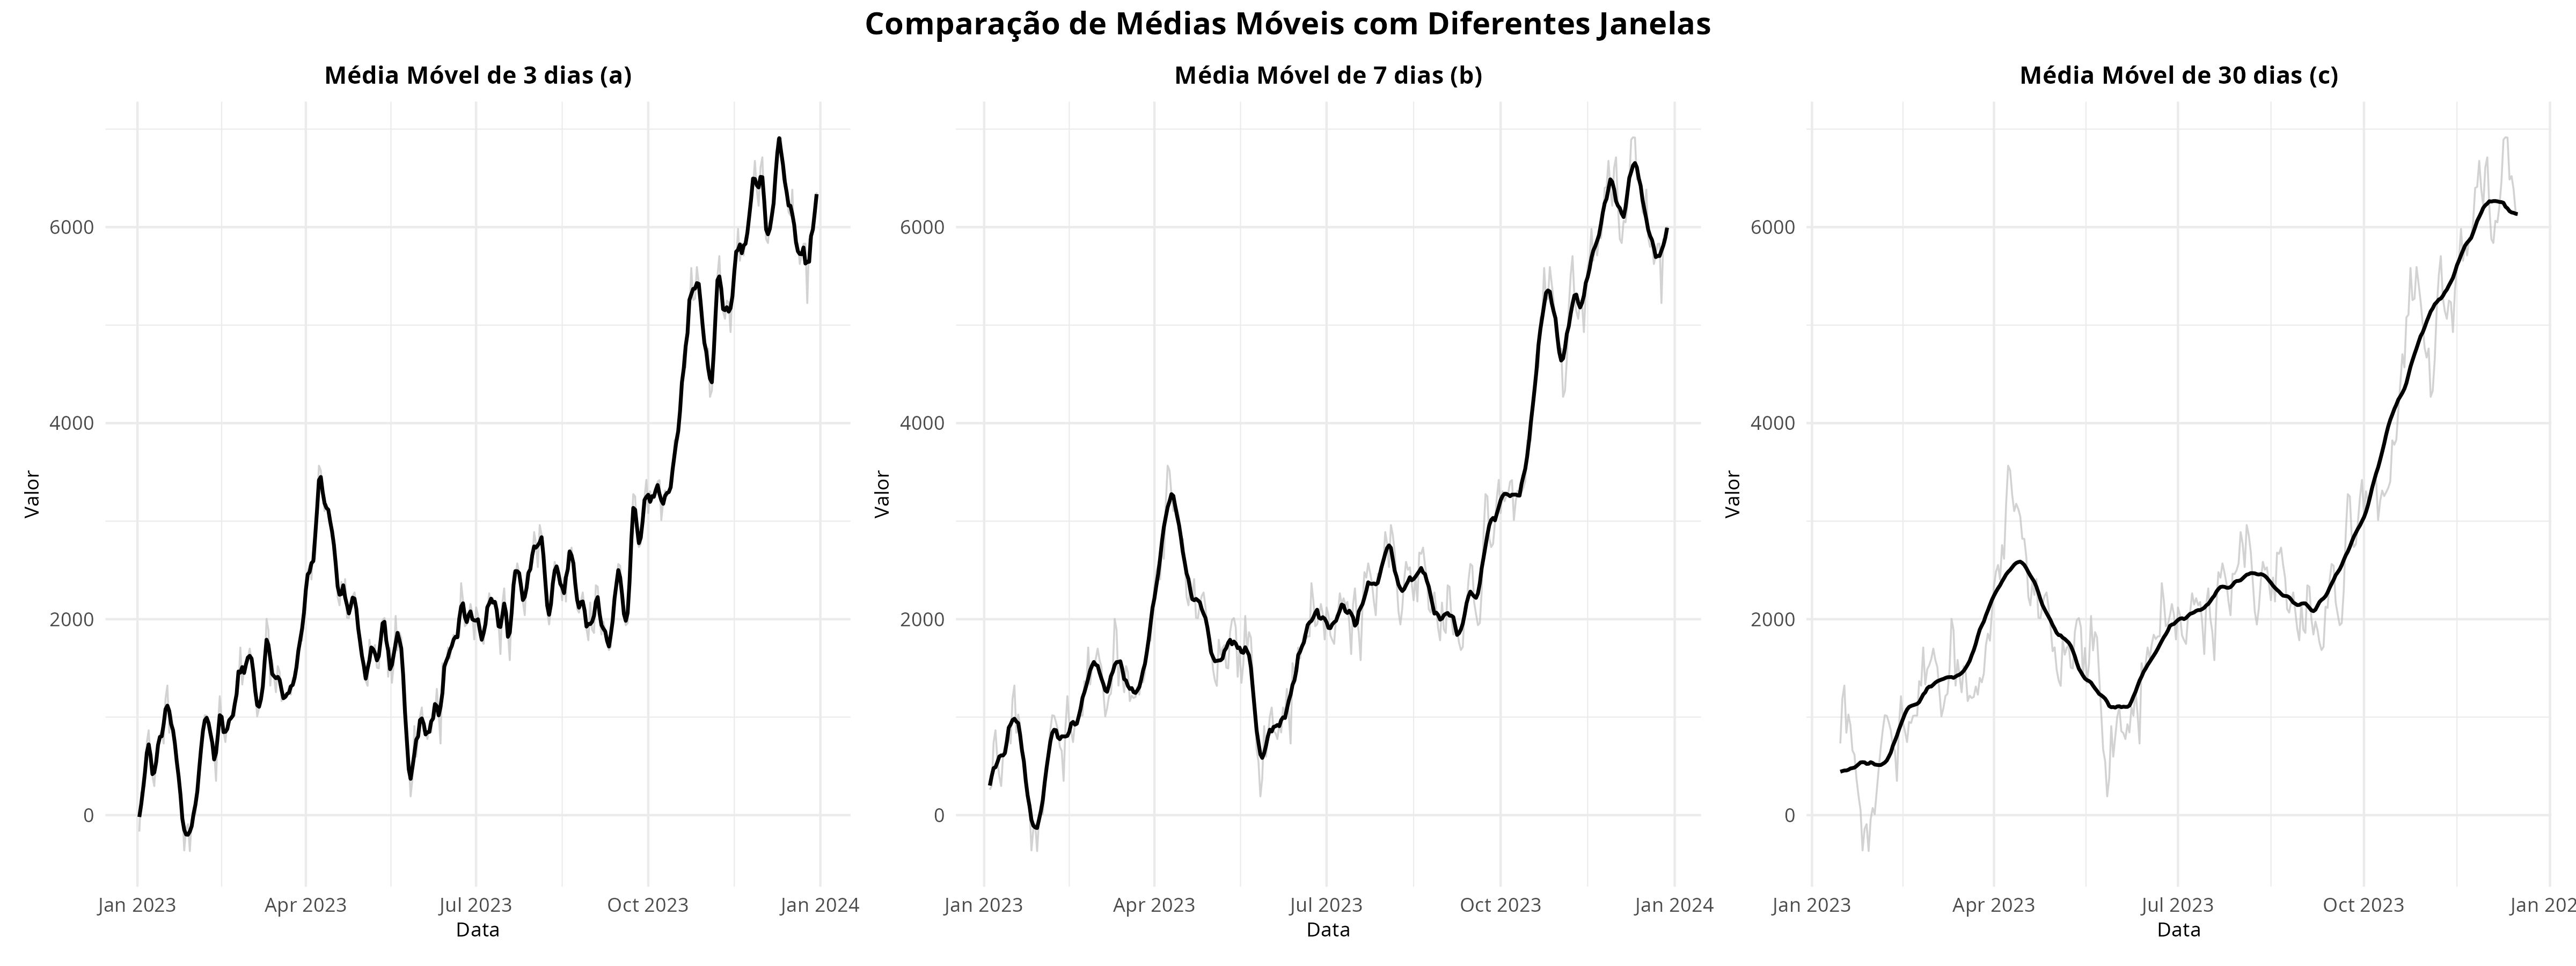
\includegraphics[width=1.0\linewidth]{medias_moveis.png}
    \caption{Suavização da série temporal por média móvel. (a) Suavização com $n = 3$ dias; (b) Suavização com $n = 7$ dias; (c) Suavização com $n = 30$ dias. Ao fundo de cada exemplo, em cinza, está plotada a série temporal sem suavização.}
    \label{fig:suavizacao_serie_temporal}
\end{figure}

A Figura \ref{fig:suavizacao_serie_temporal} apresenta a aplicação de diferentes graus de suavização em uma série. Observa-se que o aumento do grau de suavização reduz as oscilações da série, mantendo a média local.

\section{Agregação Temporal}
\label{sec:agregacao_temporal}

Uma técnica amplamente utilizada na previsão de séries temporais é a agregação temporal das observações. Transformar a série por meio de agregação temporal permite analisá-la em outros agrupamentos de tempo. Podem ser realizados agrupamentos contendo observações semanais, quinzenais ou mensais, por exemplo \citep{salles_evaluating_2016}. Estatisticamente falando, a agregação temporal atua como um mecanismo de suavização que reduz a variância dos erros de alta frequência. Ao agregar as observações, componentes sazonais de curto prazo e irregularidades tendem a se compensar, destacando os componentes de tendência e ciclo da série. É evidenciado que, quanto maior o nível de agregação temporal, mais fácil se torna a previsão de uma série temporal, apesar de ser necessária uma quantidade mínima para compor uma série agregada \citep{Rostami2013Demand, silvestrini2008temporal}.

Dada uma série temporal $x_t$, com $t = 1, 2, \dots, n$ representando os dias sequenciais, sua versão agregada $X_T$, com janela de agregação de tamanho $m$, é obtida pela fórmula \ref{eq:agregacao_temporal}, em que $T$ indica a sequência de observações da série agregada.

\begin{equation}
X_T = \sum_{t=(T-1)m + 1}^{tm} x_t, \quad \text{para } T = 1, 2, \dots, \left\lfloor \frac{n}{m} \right\rfloor
\label{eq:agregacao_temporal}
\end{equation}

\section{Modelos de Aprendizado de Máquina}
\label{sec:modelos_aprendizado_maquina}

Diferente de modelos estatísticos tradicionais, modelos de \gls{ML} em séries temporais funcionam como aproximadores universais de uma função contínua, tendo como base observações passadas. Desde que se tenha dados suficientes como base, esses modelos  são capazes de aprender com esses dados e utilizar seu conhecimento para prever os dados seguintes. Dentre os modelos de \gls{ML}, os mais conhecidos são modelos de Redes Neurais que imitam o funcionamento do cérebro humano, conectando os neurônios por meio de sinapses, as quais possuem pesos associados que representam a relevância de cada conexão \citep{ogasawara_event_2025}. 

Embora, hoje em dia, os modelos sejam bastante difundidos, eles são muito dependentes de configurações internas para que seu funcionamento seja adequado aos dados quais estão submetidos. Para ajustar essas configurações é preciso ter um nível de conhecimento um pouco maturado\citep{koutsoukas2017deep}. Essas configurações são chamadas de hiperparâmetros  quando definidas compõem uma instância única do modelo. Os hiperparâmetros podem estar olLP, ou ao número de núcleos de agrupamento, no caso do KNN, entre outros exemplos \citep{ogasawara_event_2025}.

Hiperparâmetros são variáveis fundamentais que afetam a maneira como os modelos descobrem os padrões de um conjunto de dados. A sua seleção de impacta diretamente no desempenho de um modelo. Uma técnica popularmente conhecida e utilizada para otimização de hiperparâmetros é a Busca em Grade (Grid Search). Esta técnica busca testar diversas combinações de hiperparâmetros para avaliar e escolher o um modelo mais eficiente \citep{monica2024Hyperparameter, ramamohan2024discrete}. 

\chapter{Trabalhos Relacionados}
\label{sec:trabalhos_relacionados}

A previsão de séries temporais tem sido amplamente estudada e aplicada em diferentes domínios, como finanças, saúde, indústria e gestão pública. Diversas abordagens foram propostas, desde modelos estatísticos tradicionais até técnicas mais recentes baseadas em aprendizado de máquina.

A revisão sistemática considerou publicações anteriores a 2024, com foco na previsão de receitas públicas por meio de séries temporais, utilizando os termos "previsão de receitas de multas de trânsito; previsão orçamentária" nas bases Scopus e Google Scholar. Diversos resultados foram obtidos. Observou-se que a previsão de receitas públicas é um tema bastante explorado, sobretudo em áreas periféricas, como previsão de ICMS, de infrações de trânsito e de IPVA, entre outras. Apesar de se tratar de um tema relevante no contexto do orçamento municipal, verifica-se uma baixa quantidade de estudos voltados à previsão de receitas de multas de trânsito. Apenas dois estudos com temas semelhantes foram encontrados, dos quais somente um apresenta relação direta com o objetivo deste trabalho.

\citet{pucrjreceitas} realiza previsões com a mesma serie temporal de receitas de multas de transito, porém, com um recorte do inpicio de 2019 ao final de 2023 Eles adotam, na metodologia, uma abordagem que tenta contornar impactos causadeos pela COVID-19. Para a previsão final, utilizaram o modelo SARIMA(1,1,1)-(1,1,12), que contém uma componente sazonal de 12 meses. Neste estudo não foram obtidos resultados relevantes que pudessem ser utilizados para prever efetivamente e período desejado. O ponto que mais se destaca é que os autores não realizaram experimentos com modelos mais robustos de aprendizado de máquina como MLP, KNN e ELM.

\citet{da_silva_orcamento_2018}, visando aumentar a efetividade da previsão de receitas do município de Uberlândia, realiza um estudo comparativo entre a previsão de receitas feita pela \gls{SETTRAN}, com base no modelo disponibilizado pela \gls{SOF}, e a previsão realizada com o modelo \gls{ARMA}, no período de 2002 a 2017. O estudo mostra que o modelo \gls{ARMA} utilizado foi mais preciso, com percentual médio de erros de 17{,}19\%, frente a 24{,}47\% do modelo da \gls{SOF}. Também é demonstrado que o modelo \gls{ARMA} apresentou erro médio inferior em 9 dos 16 anos analisados. Os autores não realizam qualquer tipo de transformação na série original utilizada.

Em um contexto similar, \citet{naibert_orcamento_2021} compara o desempenho da previsão de receitas de diversos municípios do estado do Rio Grande do Sul entre os anos de 2008 e 2019. O autor realiza um estudo comparativo entre o modelo da \gls{SOF} e o \gls{ARIMA}. Os resultados indicam que o modelo da \gls{SOF} é mais suscetível a erros, enquanto o \gls{ARIMA} apresenta desempenho superior em 83\% dos casos analisados. Observa-se, entretanto, que essa dominância não é uniforme. Por exemplo, no município de Porto Alegre, o modelo da \gls{SOF} foi superior em 11 dos 12 casos testados. Embora o estudo indique a superioridade do \gls{ARIMA} em relação ao modelo da \gls{SOF}, as séries utilizadas estão inseridas em contextos distintos.

De modo geral, a literatura revisada aponta um déficit na capacidade preditiva do modelo da \gls{SOF}, que apresenta desempenho inferior ao modelo \gls{ARIMA}. A previsão de receitas públicas ainda carece de soluções eficazes, o que contribui para tornar o planejamento orçamentário incerto e desatualizado. A comparação com estudos anteriores é limitada por diferenças estruturais entre as séries, particularmente no período pandêmico, que introduz quebras de padrão não modeladas nos trabalhos revisados. Diferentemente dos estudos mencionados, este trabalho explora a transformação da série temporal por suavização e agregação como mecanismo de mitigação de ruídos e de melhoria da acurácia preditiva.

\chapter{Método}
\label{sec:metodologia} 

A metodologia adotada neste trabalho propõe a realização de previsões para séries temporais de arrecadação de multas de trânsito no município do Rio de Janeiro. Ao final, os resultados obtidos são utilizados para comparar o desempenho das instâncias dos modelos. As previsões são realizadas no ambiente \textit{RStudio 2024.12.0}, com auxílio das bibliotecas \textit{TSPredit} e \textit{Daltoolbox} \citep{ogasawara_tspredit_2025, daltoolbox}. A seguir, apresenta-se a Seção \ref{sec:base_de_dados}, que fornece informações sobre o conjunto de dados. A Seção \ref{sec:implementacao} descreve as etapas de execução do trabalho. Ressalta-se que os dados utilizados referem-se exclusivamente a registros históricos de pagamentos de multas de trânsito decorrentes de multas já lavradas pelo município, não estando relacionados à definição, alteração ou proposição de políticas de multa ou de fiscalização. A finalidade da pesquisa restringe-se à análise estatística da série temporal dessas receitas, com foco na melhoria da acurácia preditiva para fins de planejamento orçamentário, e não à formulação de medidas voltadas ao aumento da arrecadação.

\section{Base de dados} 
\label{sec:base_de_dados}

Disponibilizada pela \cite{dataRioSMTR} por meio do portal de dados abertos 
\textit{Data.Rio}, a base de dados é composta por registros de infrações de trânsito no período de 2014 a 2025, contendo informações como data da ocorrência, data de pagamento, valor da infração, tipo de veículo, entre outras. Os dados estão ordenados pela data de pagamento. Neste trabalho, utilizam-se apenas os atributos \textit{Data de Pagamento}, \textit{Valor Pago} e \textit{Data de Ocorrência}.

\section{Implementação}
\label{sec:implementacao}

Na etapa inicial da implementação, ocorre o carregamento dos dados. Em seguida, realiza-se o pré-processamento, que inclui o tratamento de valores inválidos, conversões e a definição dos limites temporais da série. Nessa etapa, também são removidas as multas sem valor pago registrado, por impossibilitarem a consolidação da série de receitas efetivas, sendo tratadas como dados censurados. Como representado na Figura \ref{fig:corte_serie_temporal_2}, a série temporal de receitas diárias apresenta distorções significativas em seu início, com baixo volume de receitas em comparação ao restante da série, devido a limitações no registro das multas. Como a janela de obtenção dos dados é finita, principalmente no início da série, o cálculo de $A_{x_i}$ torna-se incerto, pois há multas pagas que não constam no conjunto disponibilizado por terem sido registradas em período anterior ao início da base. Para mitigar esse problema, realiza-se um recorte, excluindo os dados anteriores a 2016. 

\begin{figure}[!ht]
	\centering
	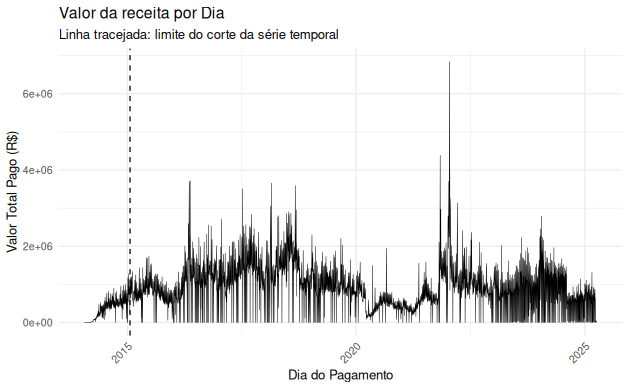
\includegraphics[width=0.6\textwidth]{figures/corte_serie_temporal.png}
	\caption{Série temporal sinalizando o início com receita reduzida devido à limitação de dados. A linha tracejada indica o limite do recorte da série.}
	\label{fig:corte_serie_temporal}
\end{figure}

Após o pré-processamento, ocorre a criação da série efetivamente utilizada para a modelagem. As multas são organizadas com agregação mensal das receitas, de forma que todas as multas pagas em um mesmo mês sejam somadas, gerando a série temporal de receitas mensais $z_i$. Para um mês específico $x_i$ no período analisado (i-ésimo mês), o valor da receita mensal $z_i$ é calculado pela soma dos valores individuais $y_k$ de todas as $n$ multas que compõem o conjunto $A_{x_i}$ (todas as multas pagas nesse mês). A equação da série é definida pela Equação \ref{eq:formula serie receita}:

\begin{equation}
    z_i = \sum_{k=1}^{n} y_k \quad \text{para cada} \quad a_k \in A_{x_i}
    \label{eq:formula serie receita}
\end{equation}

Posteriormente à criação da série de receitas mensais, obtém-se um dataframe que será armazenado para servir como input na etapa seguinte. O dataframe contém apenas o valor arrecadado no mês, e constam exatamente 120 meses de arrecadação, do início de 2016 ao final de 2024.

Na implementação, utiliza-se e adapta-se um framework de experimentação exaustiva que emprega a técnica de \textit{Grid Search} para otimização de hiperparâmetros. Seu propósito central é iterar sobre combinações de um conjunto pré-definido de hiperparâmetros, treinar os modelos com essas combinações, em seguida testar os modelos e registrar suas métricas de avaliação. É importante mencionar que, embora configurações como métodos de normalização, tamanho da janela deslizante (\textit{sliding window}) e tamanho das janelas de treino e teste sejam padronizadas para todos os experimentos, os \textit{ranges} (parâmetros particulares de cada modelo) dos principais hiperparâmetros são únicos para cada modelo. Por exemplo, o modelo \gls{MLP} varia em \textit{input\_size} e \textit{size} (camadas internas), enquanto o \gls{KNN} varia no número $k$ de vizinhos próximos. A seguir, apresenta-se um pseudocódigo que representa o processo realizado pelo framework.

A função \textit{run\_ml} é utilizada para iniciar o processo. Ela é responsável por armazenar todos os casos de combinações de hiperparâmetros possíveis e repassar para as funções intermediárias que irão treinar e testar o modelo com janelas deslizantes variáveis. Para treinar os casos dos modelos, avalia-se e mensura-se qual caso obtém o melhor ajuste possível, com base na métrica de erro. Quanto menor o erro, melhor o desempenho do modelo. No teste, o modelo é testado em um período sequencial de 12 meses (um ano à frente). Por fim, a lista com todos os modelos é retornada e ordenada para identificar o melhor desempenho de cada modelo.

\begin{algorithm}
\caption{run\_ml}
\label{alg:main_experiment}
\begin{algorithmic}[1]
\State $\text{df} \gets \text{carregar\_dataframe()}$
\State $\text{ts} \gets \text{obter\_serie(df)}$
\State $\text{t\_teste} \gets \text{12}$
\State $\text{t\_treino} \gets \text{obter\_tamanho\_serie(ts) - tamanho\_teste}$
\State $\text{combinacoes} \gets \text{obter\_combinacoes(preprocs, hiperparametros)}$
\State $\text{resultados\_gerais} \gets \text{nova\_lista()}$
\For{caso \textbf{em} combinações}
    \State $\text{modelo\_otimizado} \gets \text{treinar\_ml(ts[1:t\_treino], caso, t\_janela)}$
    \State $\text{resultado\_teste} \gets \text{testar\_ml}(\text{modelo\_otimizado}, \text{ts}, \text{t\_treino} + 1, \text{t\_teste}, \text{t\_teste})$
    \State $\text{resultados\_gerais} \gets \text{Adicionar(resultado\_teste, resultados\_gerais)}$
\EndFor
\State $\text{resultados\_gerais} \gets \text{Ordenar(resultados\_gerais)}$
\State \textbf{RETORNAR} $\text{resultados\_gerais}$
\end{algorithmic}
\end{algorithm}

A função $treinar\_ml$ é utilizada para treinar os modelos de aprendizado de máquina. Nesta função, a série é separada em janelas e são realizados os ajustes para as diferentes combinações de parâmetros. Em seguida, verifica-se se o $smape$ é o menor dentre todas as configurações passadas, e retorna-se o melhor modelo. Com o melhor modelo, é realizado o teste com \textit{steps ahead} de 12 meses. 

\begin{algorithm}
\caption{treinar\_ml}
\label{alg:train_ml}
\begin{algorithmic}[1]
\Function{treinar\_ml}{ts, params, janelas}
    \State $\text{melhor\_erro\_global} \gets \infty$
    \State $\text{melhor\_modelo} \gets \text{NULL}$
    \For{janela \textbf{em} $\text{janelas}$}
        \State $\text{ts\_janelas} \gets \text{transformar\_em\_janelas(ts, janela)}$
        \State $\text{ts\_projecao} \gets \text{projecao\_janelas(ts\_janelas)}$
        \For{\textbf{preproc} \textbf{em} $\text{params.preprocess}$}
            \State $\text{modelo\_treinado} \gets \text{ajustar\_diretamente(ts\_projecao.input, ts\_projecao.output)}$
            \State $\text{ajuste} \gets \text{prever(modelo\_treinado, ts\_projecao.input)}$
            \State $\text{erro\_smape} \gets \text{avaliar\_smape(ts\_projecao.output, ajuste)}$
            \If{$\text{erro\_smape} < \text{melhor\_erro\_global}$}
                \State $\text{melhor\_erro\_global} \gets \text{erro\_smape}$
                \State $\text{melhor\_modelo} \gets \text{modelo\_treinado}$
            \EndIf
        \EndFor
    \EndFor
    \State \textbf{RETORNAR} $\text{melhor\_modelo}$
\EndFunction
\end{algorithmic}
\end{algorithm}

A função \textbf{testar\_ml} tem como objetivo validar o desempenho do melhor modelo selecionado na função anterior, aplicando a predição a um período definido pelo \textbf{steps\_ahead}. Para isso, ela organiza os dados de teste em janelas deslizantes e os projeta em amostras de entrada e saída, executa a previsão do \textbf{steps\_ahead} e compara os resultados previstos com os valores reais da séri. Ao final, é calculada métricas de erro, como MSE, SMAPE e $R^2$, inserindo esses indicadores em um dataframe para permitir a análise do modelo.

\begin{algorithm}
\caption{testar\_ml}
\label{alg:test_ml}
\begin{algorithmic}[1]
\Function{testar\_ml}{modelo, ts, t\_pos, t\_size, steps\_ahead}
    \State $\text{test\_data} \gets \text{x[t\_pos : t\_pos + t\_size - 1]}$
    \State $\text{xwt} \gets \text{transformar\_dados\_teste\_em\_janelas(x[janela\_relevante], obj.sw\_size)}$
    \State $\text{xyt} \gets \text{projetar\_janelas\_para\_entrada\_saida}(\text{xwt})$
    \State $\text{predicao} \gets \text{predict(obj.model, xyt.input[1,:], steps\_ahead=t\_size)}$
    \State $\text{performance} \gets \text{compute\_performance}(\text{obj.model}, \text{test\_data}, \text{predicao})$
    \State $\text{dataframe\_de\_resultados} \gets \text{Criar dataframe com as médias de MSE, SMAPE, R}^2\text{.}$
    \State \textbf{RETORNAR} $\text{dataframe\_de\_resultados}$ e $\text{objeto\_modelo\_completo}$
\EndFunction
\end{algorithmic}
\end{algorithm}

Os modelos são testados com um conjunto amplo de hiperparâmetros para que, quando combinados na busca exaustiva, seja encontrada uma quantidade de configurações suficiente para avaliar a capacidade do modelo de prever a série temporal. 
Exceto pelo Auto Arima, há parâmetros em comum entre os modelos. Todos foram testados com um conjunto de janelas de \textbf{6, 12, 24, 36 e 48} meses, que representam variações semestral e anuais; os métodos de pré-processamento utilizados foram: \textbf{ts\_norm\_an, ts\_norm\_ean, ts\_norm\_gminmax, ts\_norm\_swminmax, ts\_norm\_diff}. Na tabela \ref{tab:tabela_modelos} constam os outros modelos utilizados e o restante dos parâmetros. As notações a seguir e \textbf{seq(0.1, 0.2, 0.02)} referem-se a métodos de geração de sequências numéricas. A expressão em colchetes com dois pontos \textbf{([1:16])} indica um intervalo de números inteiros com incremento unitário; por exemplo, [1:16] define que o modelo será testado com todos os valores inteiros de 1 a 16. Já a função \textbf{seq(início, fim, incremento)} permite criar sequências com maior precisão decimal: no caso de seq(0.1, 0.2, 0.02), o parâmetro decay assume os valores 0.10, 0.12, ... , 0.20. Essas definições são fundamentais para delimitar o espaço de busca, garantindo que o algoritmo explore tanto variações discretas na arquitetura quanto ajustes finos em parâmetros de regularização.

\begin{table}[!ht]
    \centering
    \caption{Hiperparâmetros dos modelos}
    \begin{tabular}{c c} 
        \hline
        \textbf{modelo} & \textbf{configurações} \\
        \hline
        mlp & input\_size: NA;  size = [1:16];  decay = seq(0.1, 0.2, 0.02);  maxit = 1000;  
        \\
        elm & nhid = [1:18]; actfun = ['sig','relu','purelin'];
        \\
        knn & k = [3:36];
        \\
        \hline
    \end{tabular}
    \label{tab:tabela_modelos}
\end{table}

Após a execução da busca em grade, escolhe-se o melhor modelo, para o qual será criado o gráfico de uma validação cruzada com a janela do modelo. O objetivo é analisar o comportamento do modelo à medida que os dados são acrescentados, verificando a qualidade e o que é esperado dos ajustes e das predições dentro do contexto do trabalho. 

\chapter{Resultados}
\label{sec:resultados}

Esta seção apresenta e compara os resultados obtidos na experimentação, conforme] organizados na Tabela \ref{tab:tabela_resultados}. A métrica \gls{R2} foi priorizada como critério de ranqueamento por representar a proporção da variância explicada pelo modelo, sendo adequada para avaliar previsões com foco em explicabilidade global \citep{chicco_coefficient_2021}. Para os gráficos utilizados, a linha listrada em azul indica o ajuste do modelo à série temporal, enquanto a linha em verde indica os valores previstos para os 12 meses seguintes. Os resultados foram sintetizados com as três melhores configurações dos modelos testados.

\begin{table}[!ht]
    \centering
    \caption{Resultados obtidos na experimentação ranqueados em ordem crescente de $\boldsymbol{R^2}$.}
    \begin{tabular}{c c c c c c c}
         \textbf{modelo} & $\boldsymbol{R^2}$ & \textbf{SMAPE} & \textbf{MSE} \\
        \hline
        %mlp & input: 36; size: 1; decay: 0.14; maxit: 1000; & gminmax & 36 & 60.26\% & 17.43\% & $2{,}983\times10^{13}$ 
        mlp & 60.26\% & 17.43\% & $2{,}983\times10^{13}$ 
        \\ 
        %elm & nhid: 5; actfun: relu; & diff & 36 & 33.83 & 26.76 & $4{,}968\times10^{13}$  
        elm & 33.83\% & 26.76\% & $4{,}968\times10^{13}$  
        \\
        %knn & k: 19; & gminmax & 36 & 0.55\% & 21.05 & $3{,}374\times10^{13}$  
        knn & 0.55\% & 21.05\% & $3{,}374\times10^{13}$  
        \\
        auto arima & -14.02\% & 36.11\% & $8{,}561\times10^{13}$
        \\
        \hline
    \end{tabular}i
    \label{tab:tabela_resultados}
\end{table}

Tendo como base a tabela \ref{tab:tabela_resultados} e a figura \ref{fig:arima12meses}, o ARIMA apresenta ajustes bastante precisos, porém, defasados. A capacidade de explicativa deste modelo mostra uma concreta inferioridade em relação ao MLP e ELM. O seu resultado de $R^2$ negativo é compatível com um modelo que falha em capturar a variância da série original.

Para estes modelos testados, observa-se que o modelo MLP apresentou melhor desempenho para a métrica $R^2$, apesar de precisar de uma janela menor para prever série. Embora nas figuras \ref{fig:mlp12mesesfold1}, \ref{fig:mlp12mesesfold2} e \ref{fig:mlp12mesesfold3}, quando o modelo tem menores quantidades de dados de treinamento, a previsão se comporta de maneira destoante da série original, porém, no último fold (figura \ref{fig:mlp12mesesfold4}), a previsão apresenta um comportamento adequado, prevendo de forma satisfatória a média local da série original.

\begin{figure}[!ht]
	\centering
	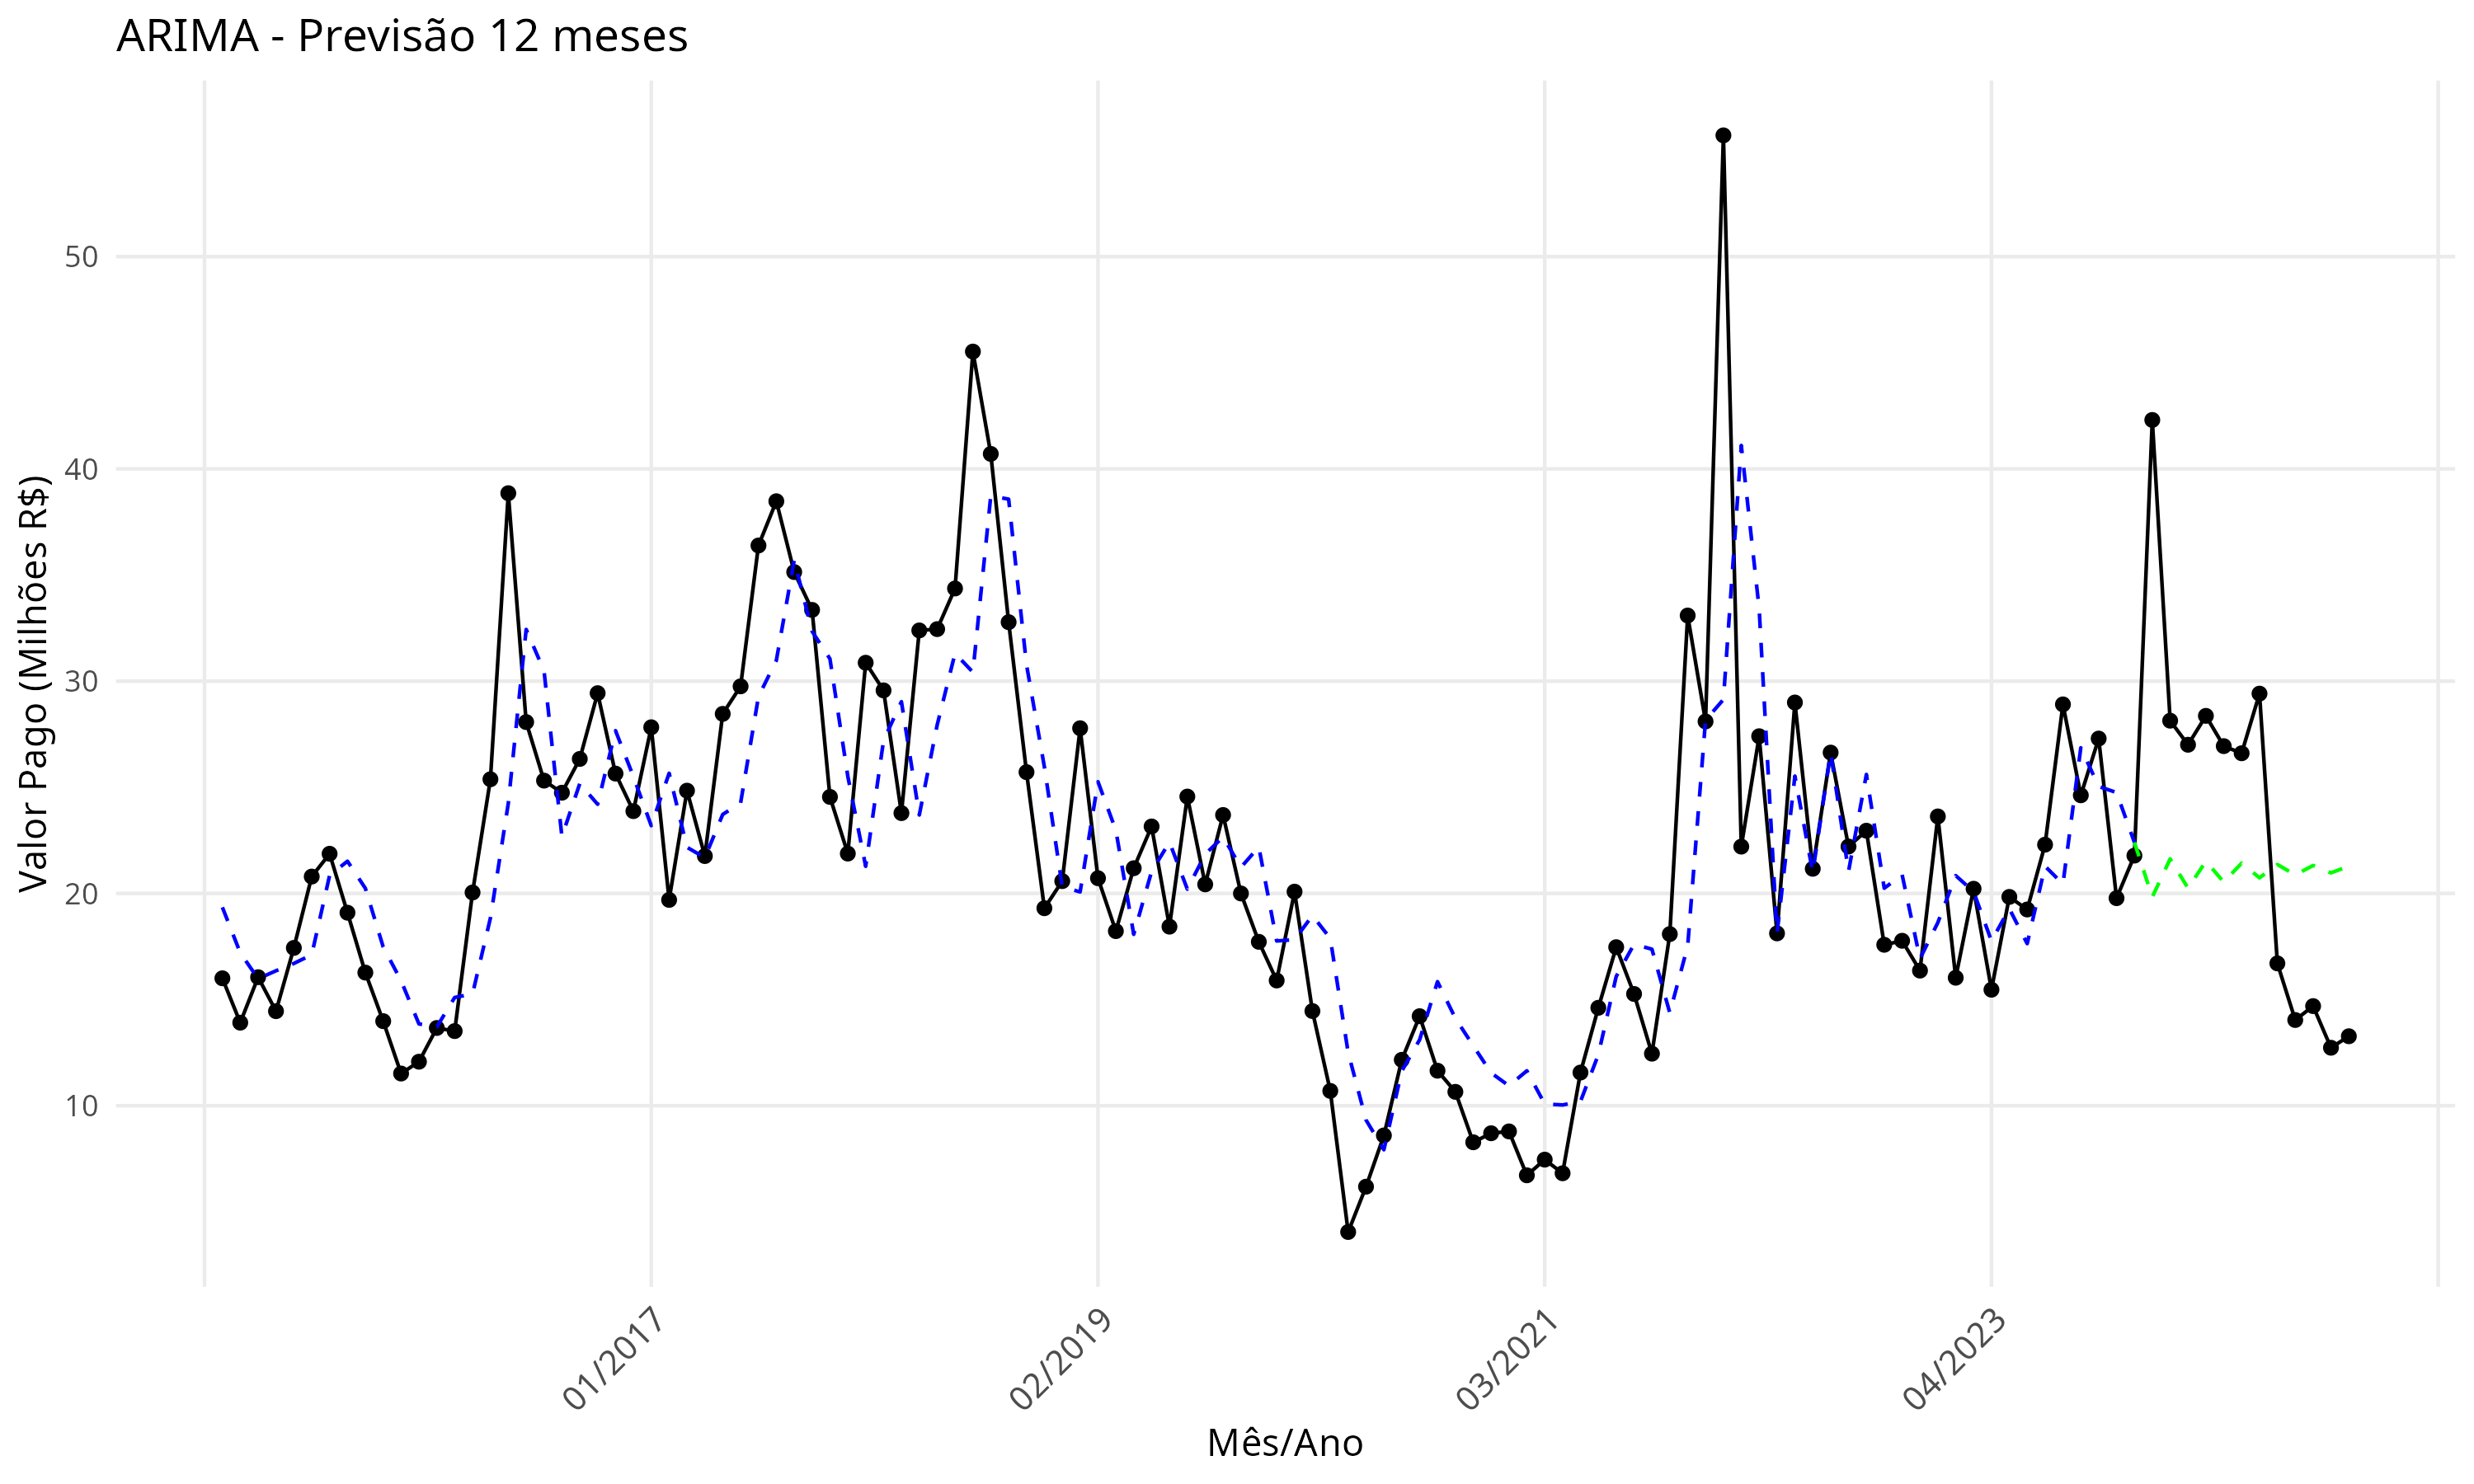
\includegraphics[width=0.8\textwidth]{figures/arima_previsao_final.png}
	\caption{Previsão da receita no período de 12 meses com o modelo Auto ARIMA.}
	\label{fig:arima12meses}
\end{figure}

\begin{figure}[!ht]
	\centering
	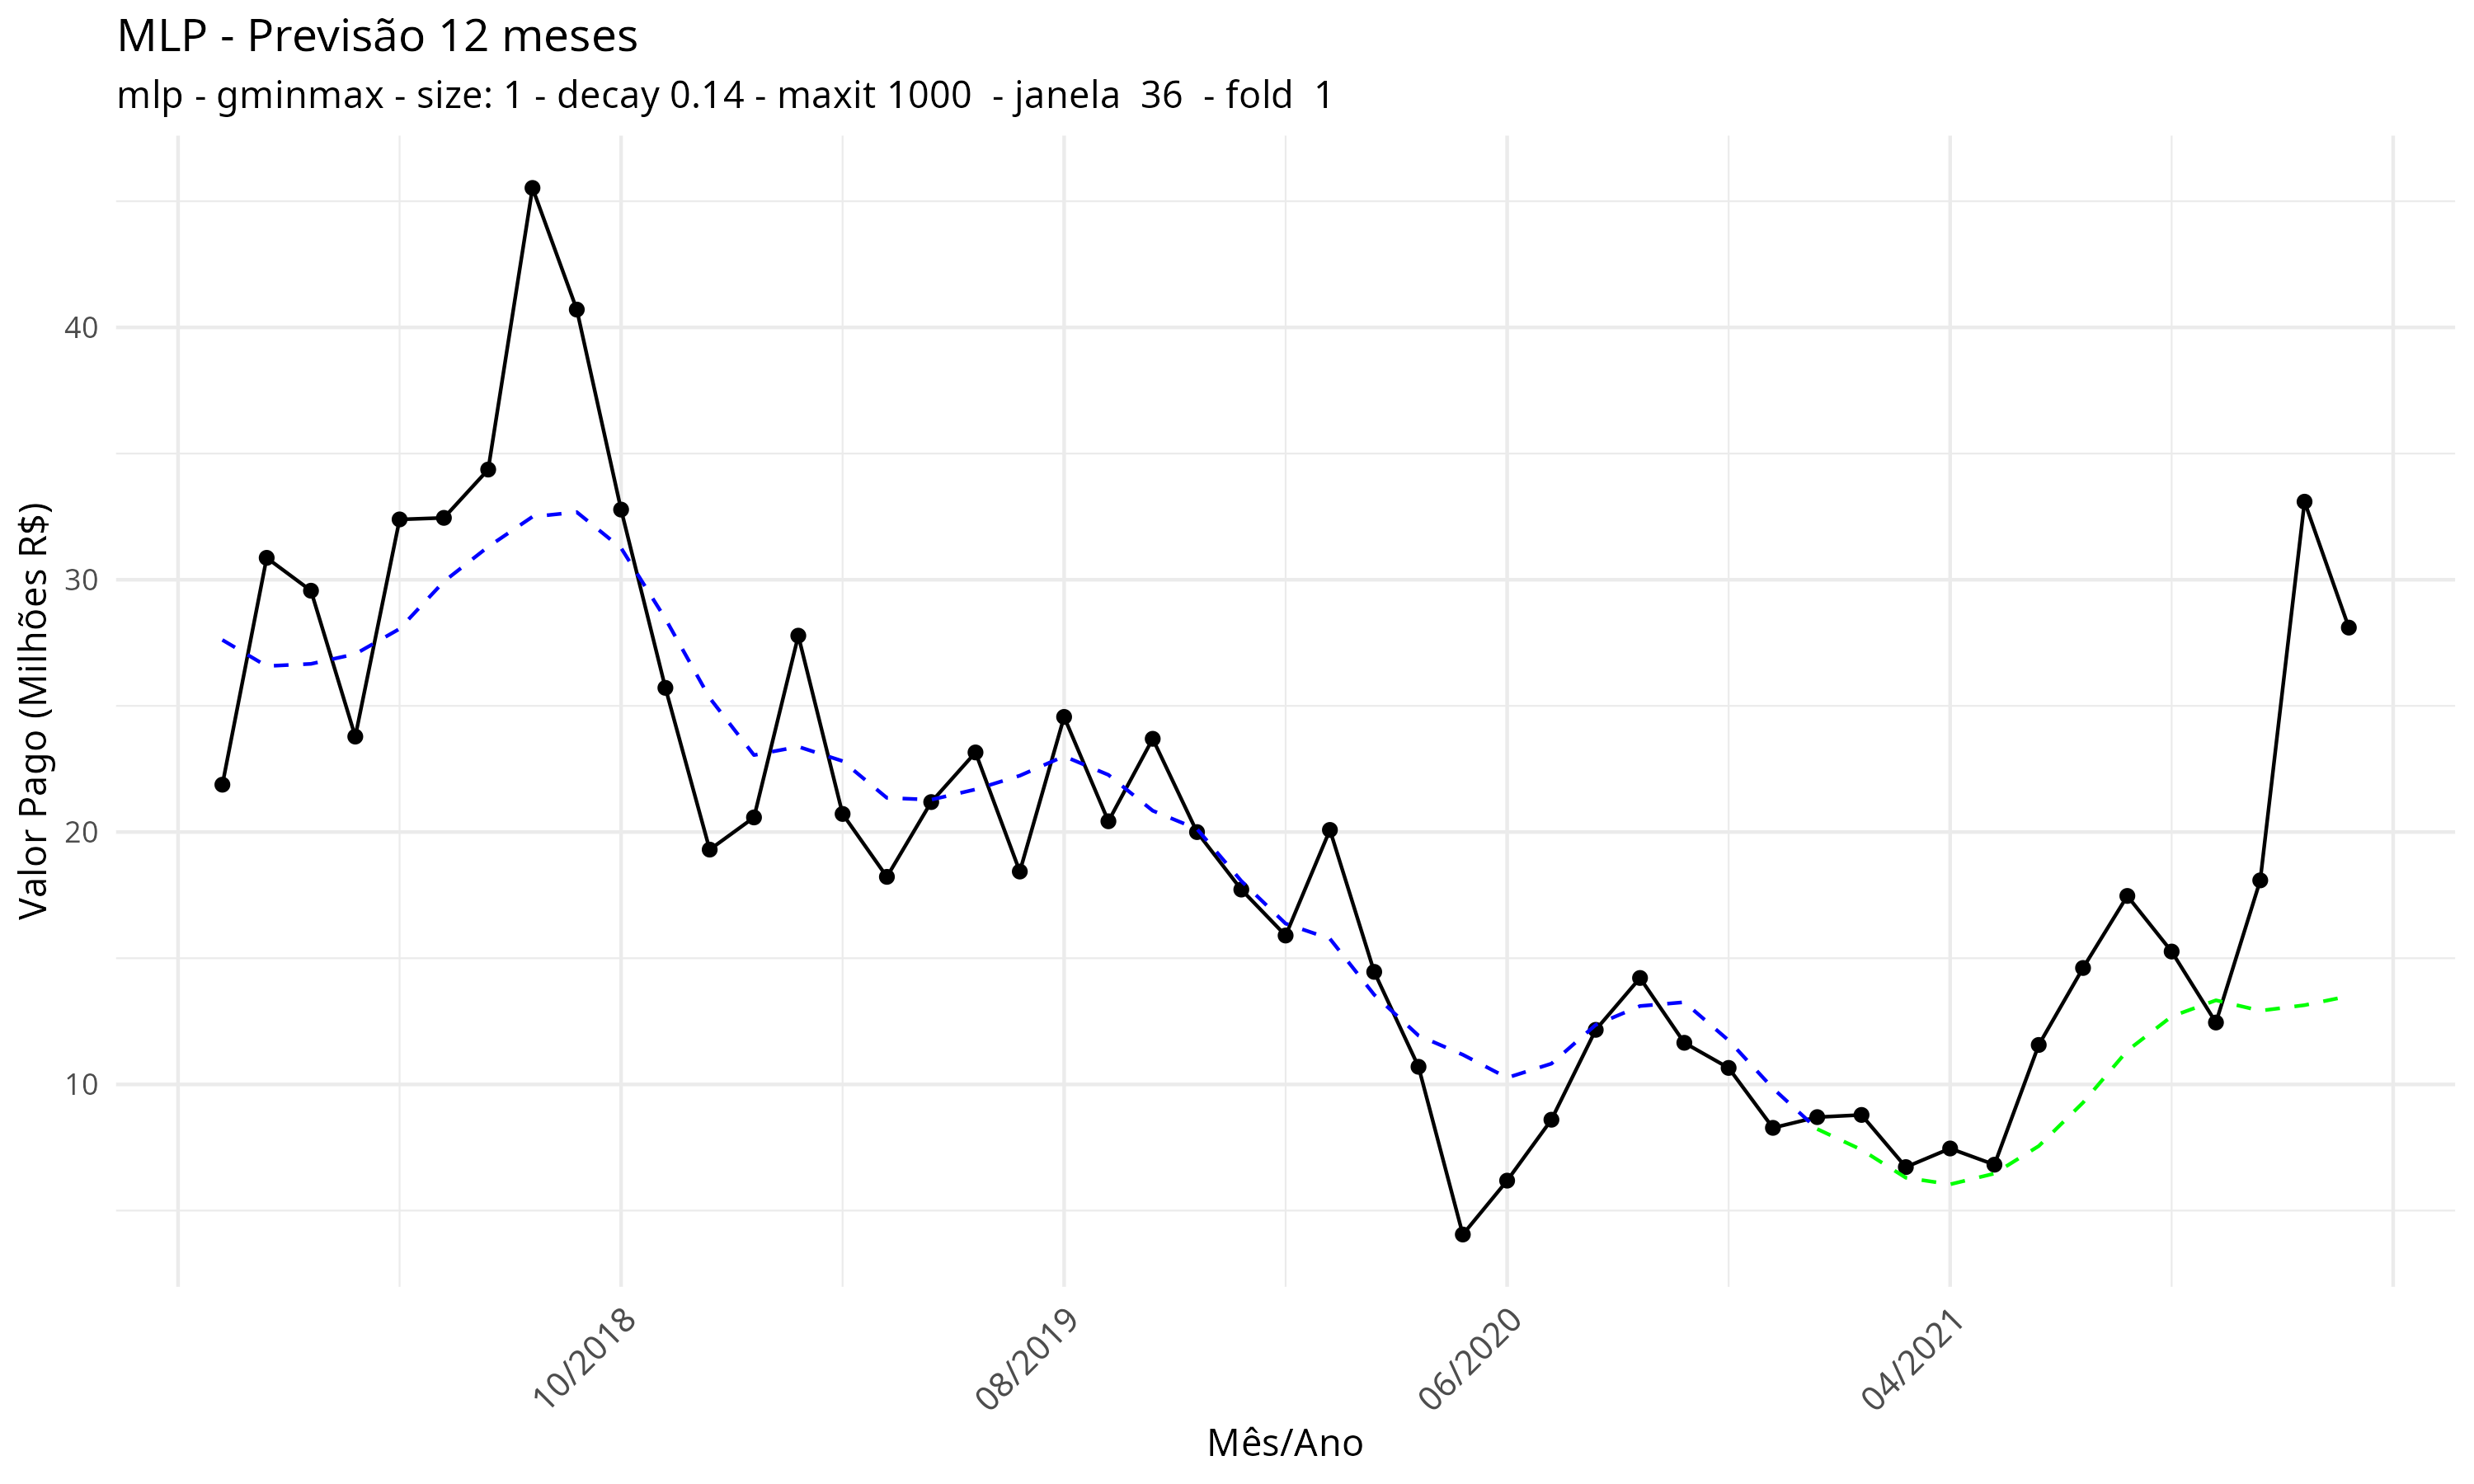
\includegraphics[width=0.8\textwidth]{figures/mlp-gminmax-s1-d014-m1000_janela-36_fold-1_plot.png}
	\caption{Previsão da receita no período de 12 meses com o modelo MLP - fold 1.}
	\label{fig:mlp12mesesfold1}
\end{figure}

\begin{figure}[!ht]
	\centering
	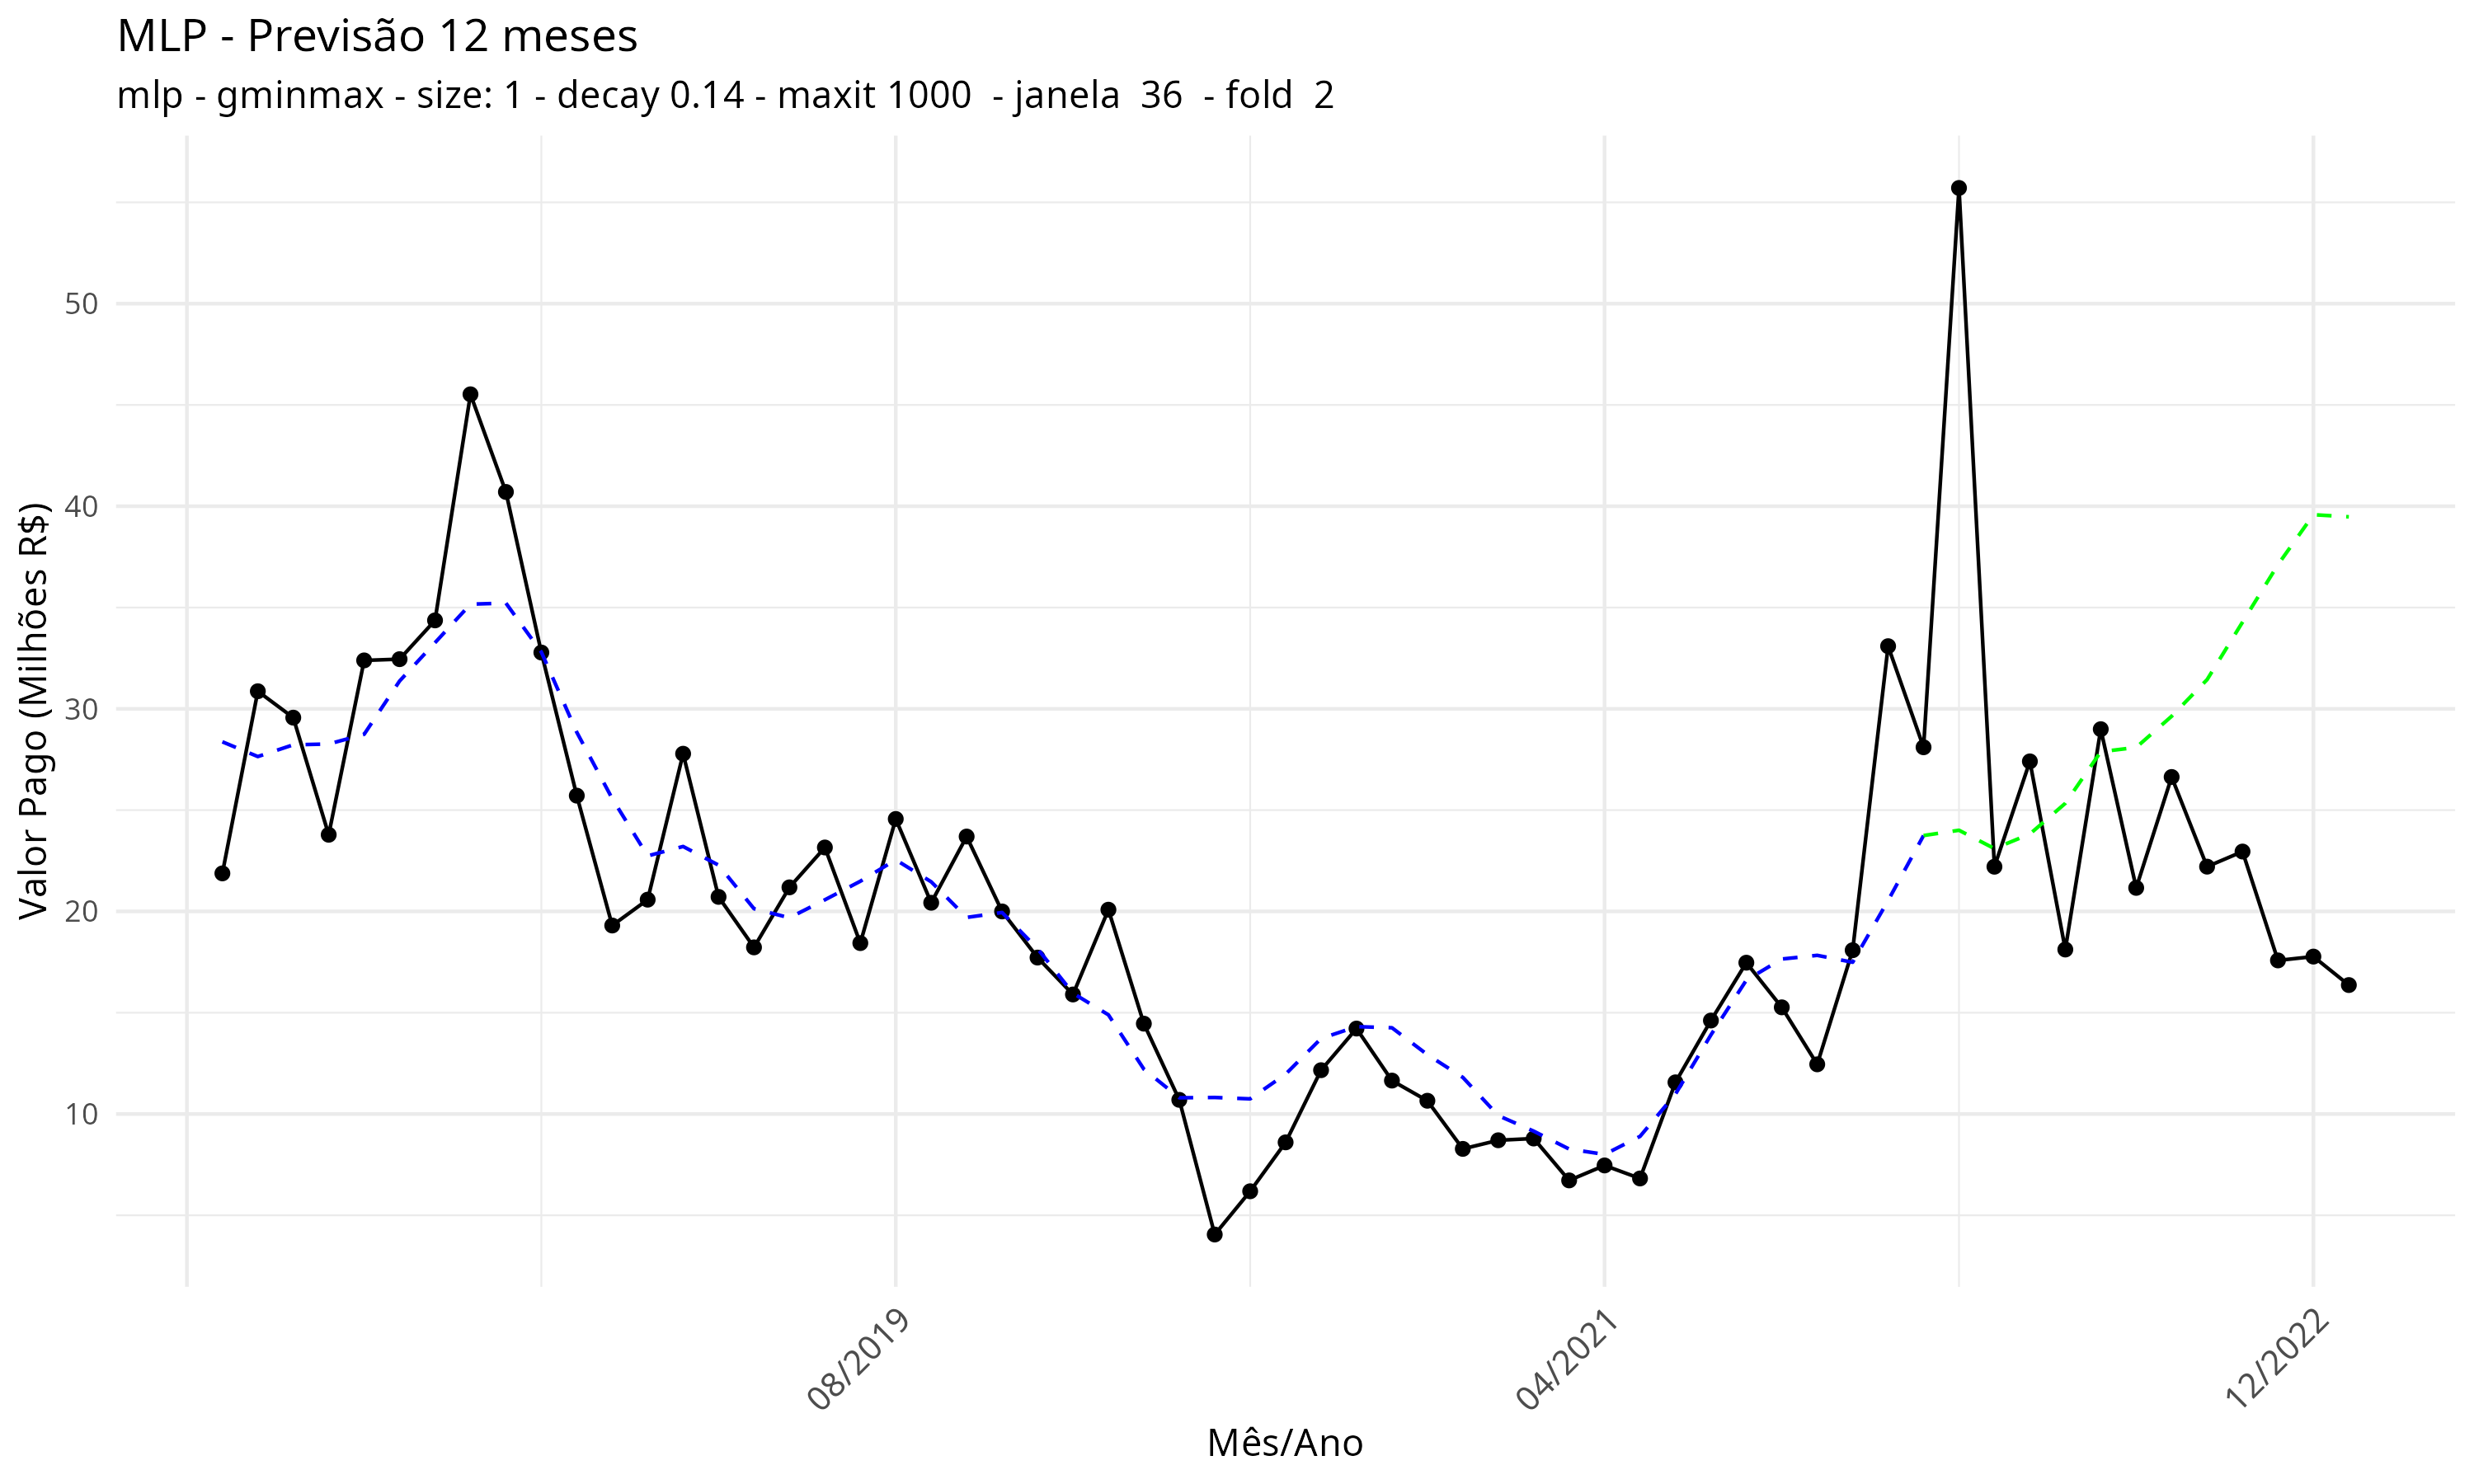
\includegraphics[width=0.8\textwidth]{figures/mlp-gminmax-s1-d014-m1000_janela-36_fold-2_plot.png}
	\caption{Previsão da receita no período de 12 meses com o modelo MLP - fold 2.}
	\label{fig:mlp12mesesfold2}
\end{figure}

\begin{figure}[!ht]
	\centering
	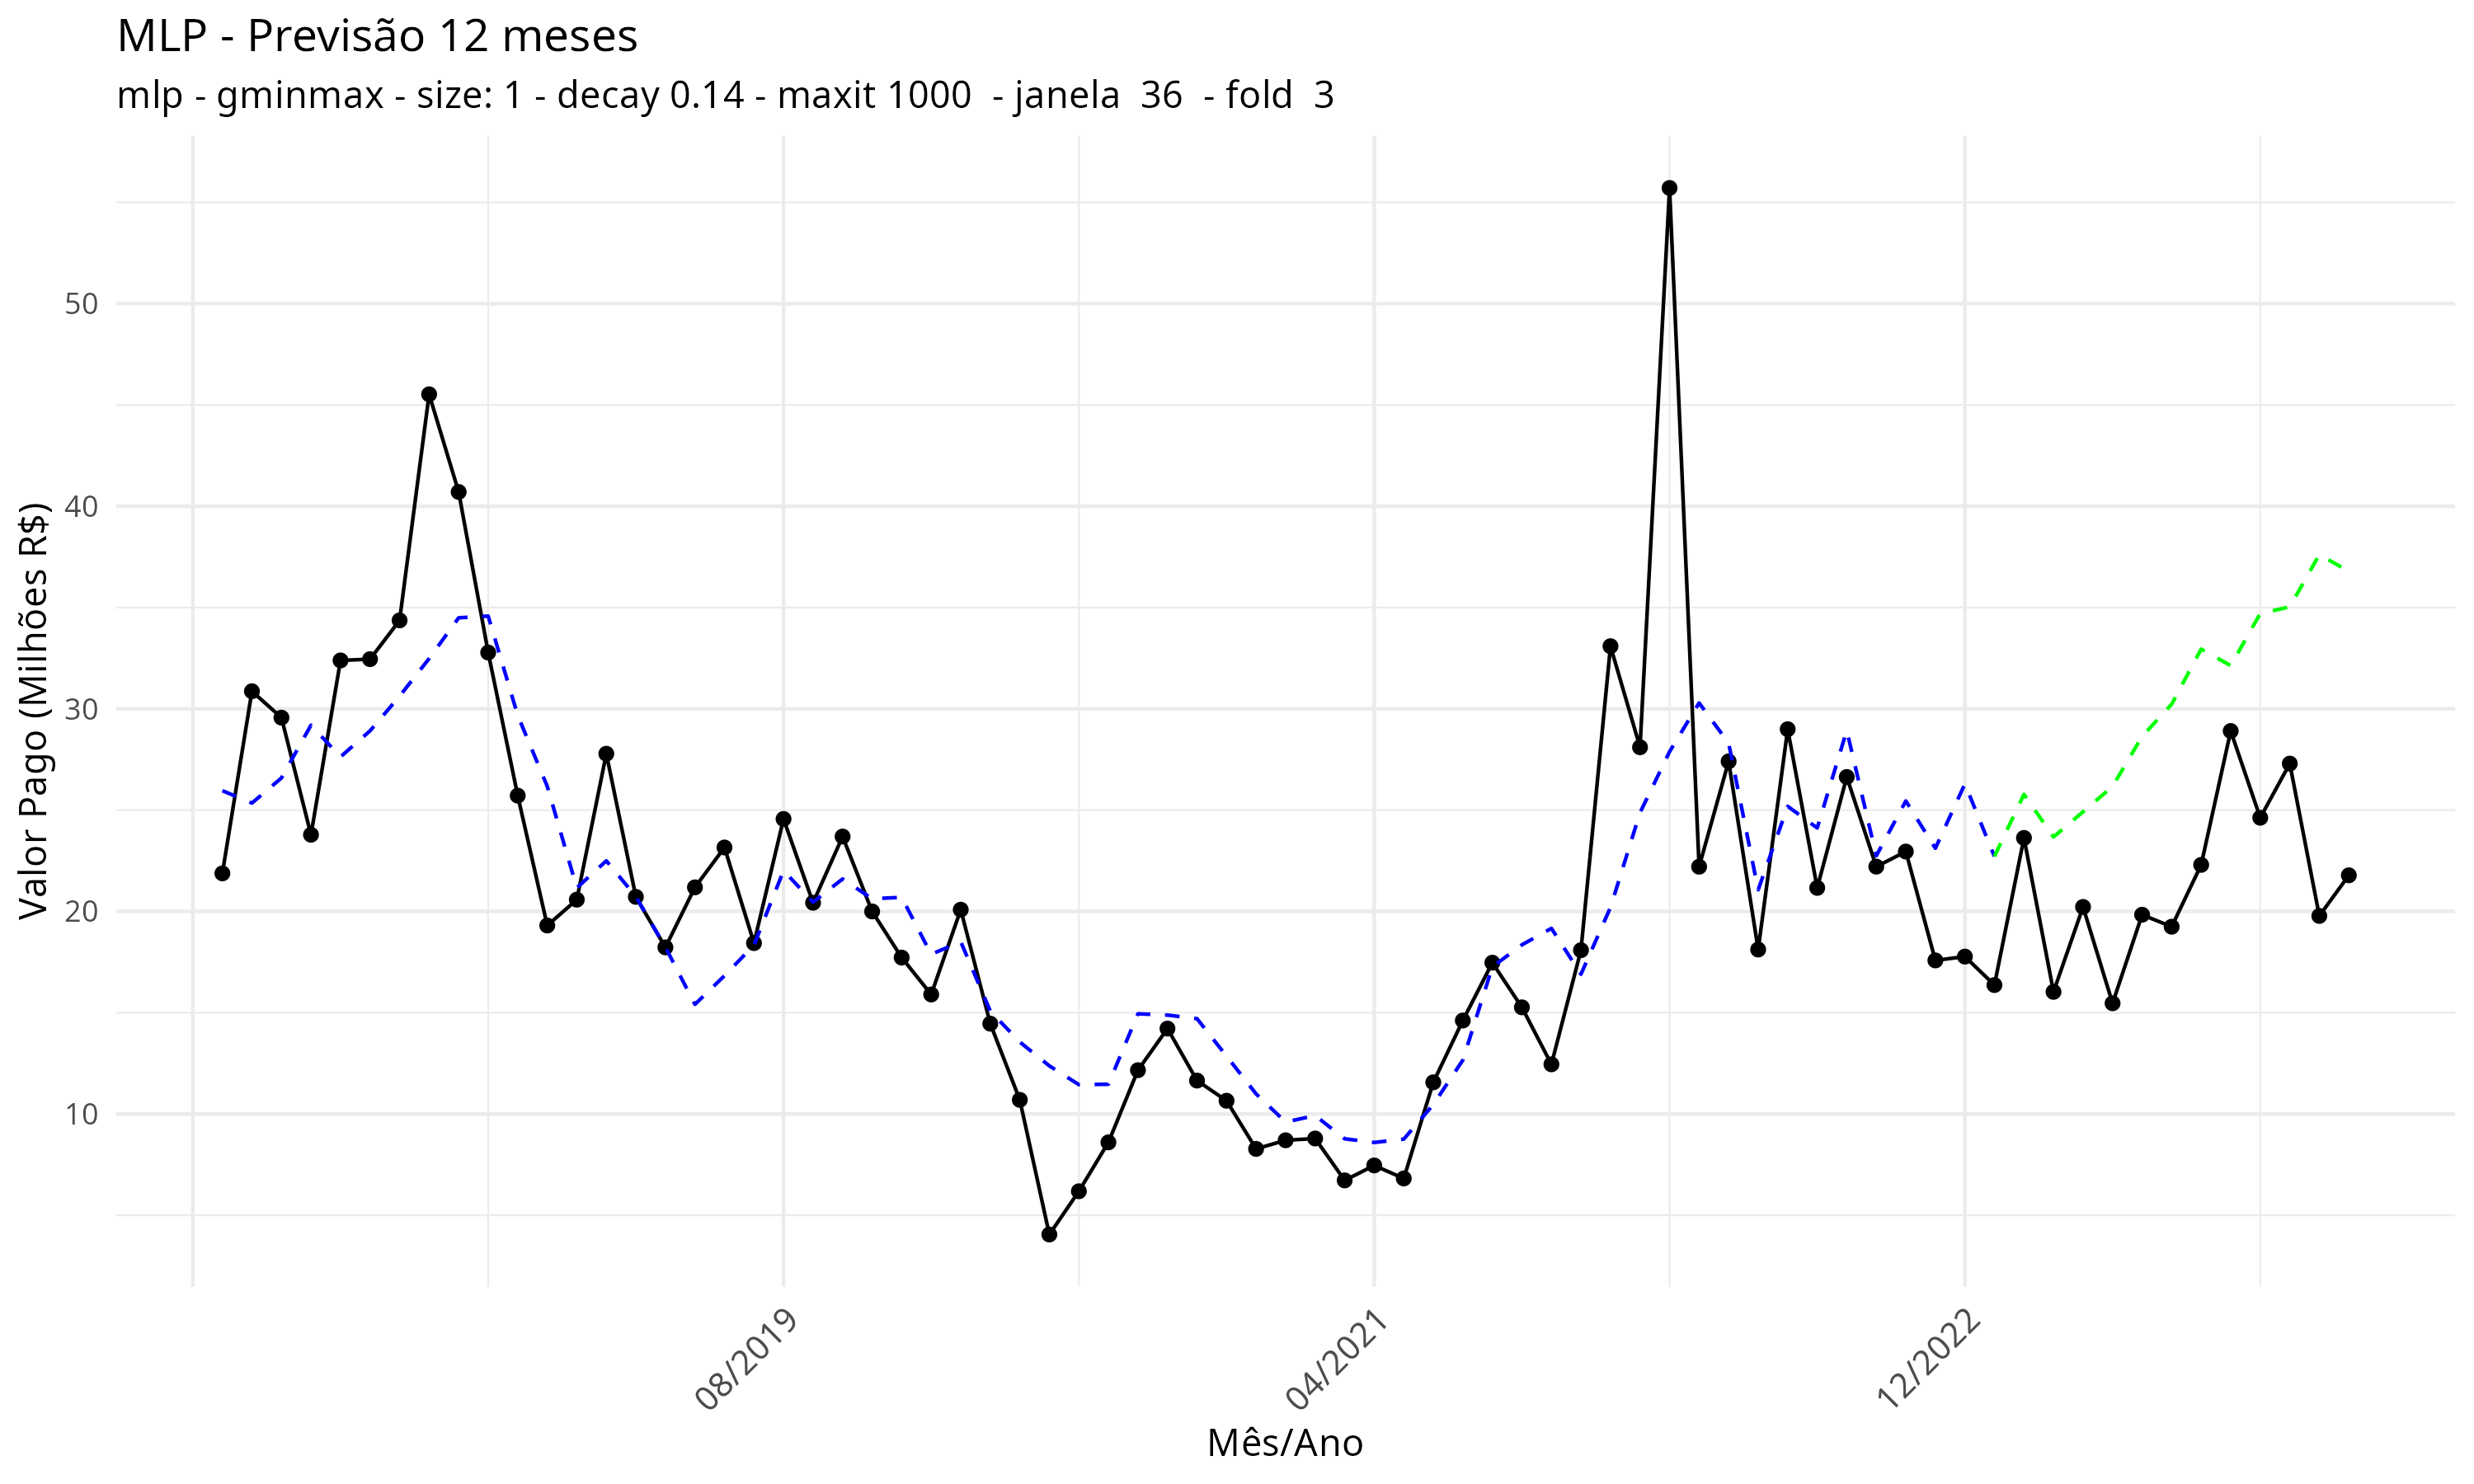
\includegraphics[width=0.8\textwidth]{figures/mlp-gminmax-s1-d014-m1000_janela-36_fold-3_plot.png}
	\caption{Previsão da receita no período de 12 meses com o modelo MLP - fold 3.}
	\label{fig:mlp12mesesfold3}
\end{figure}

\begin{figure}[!ht]
	\centering
	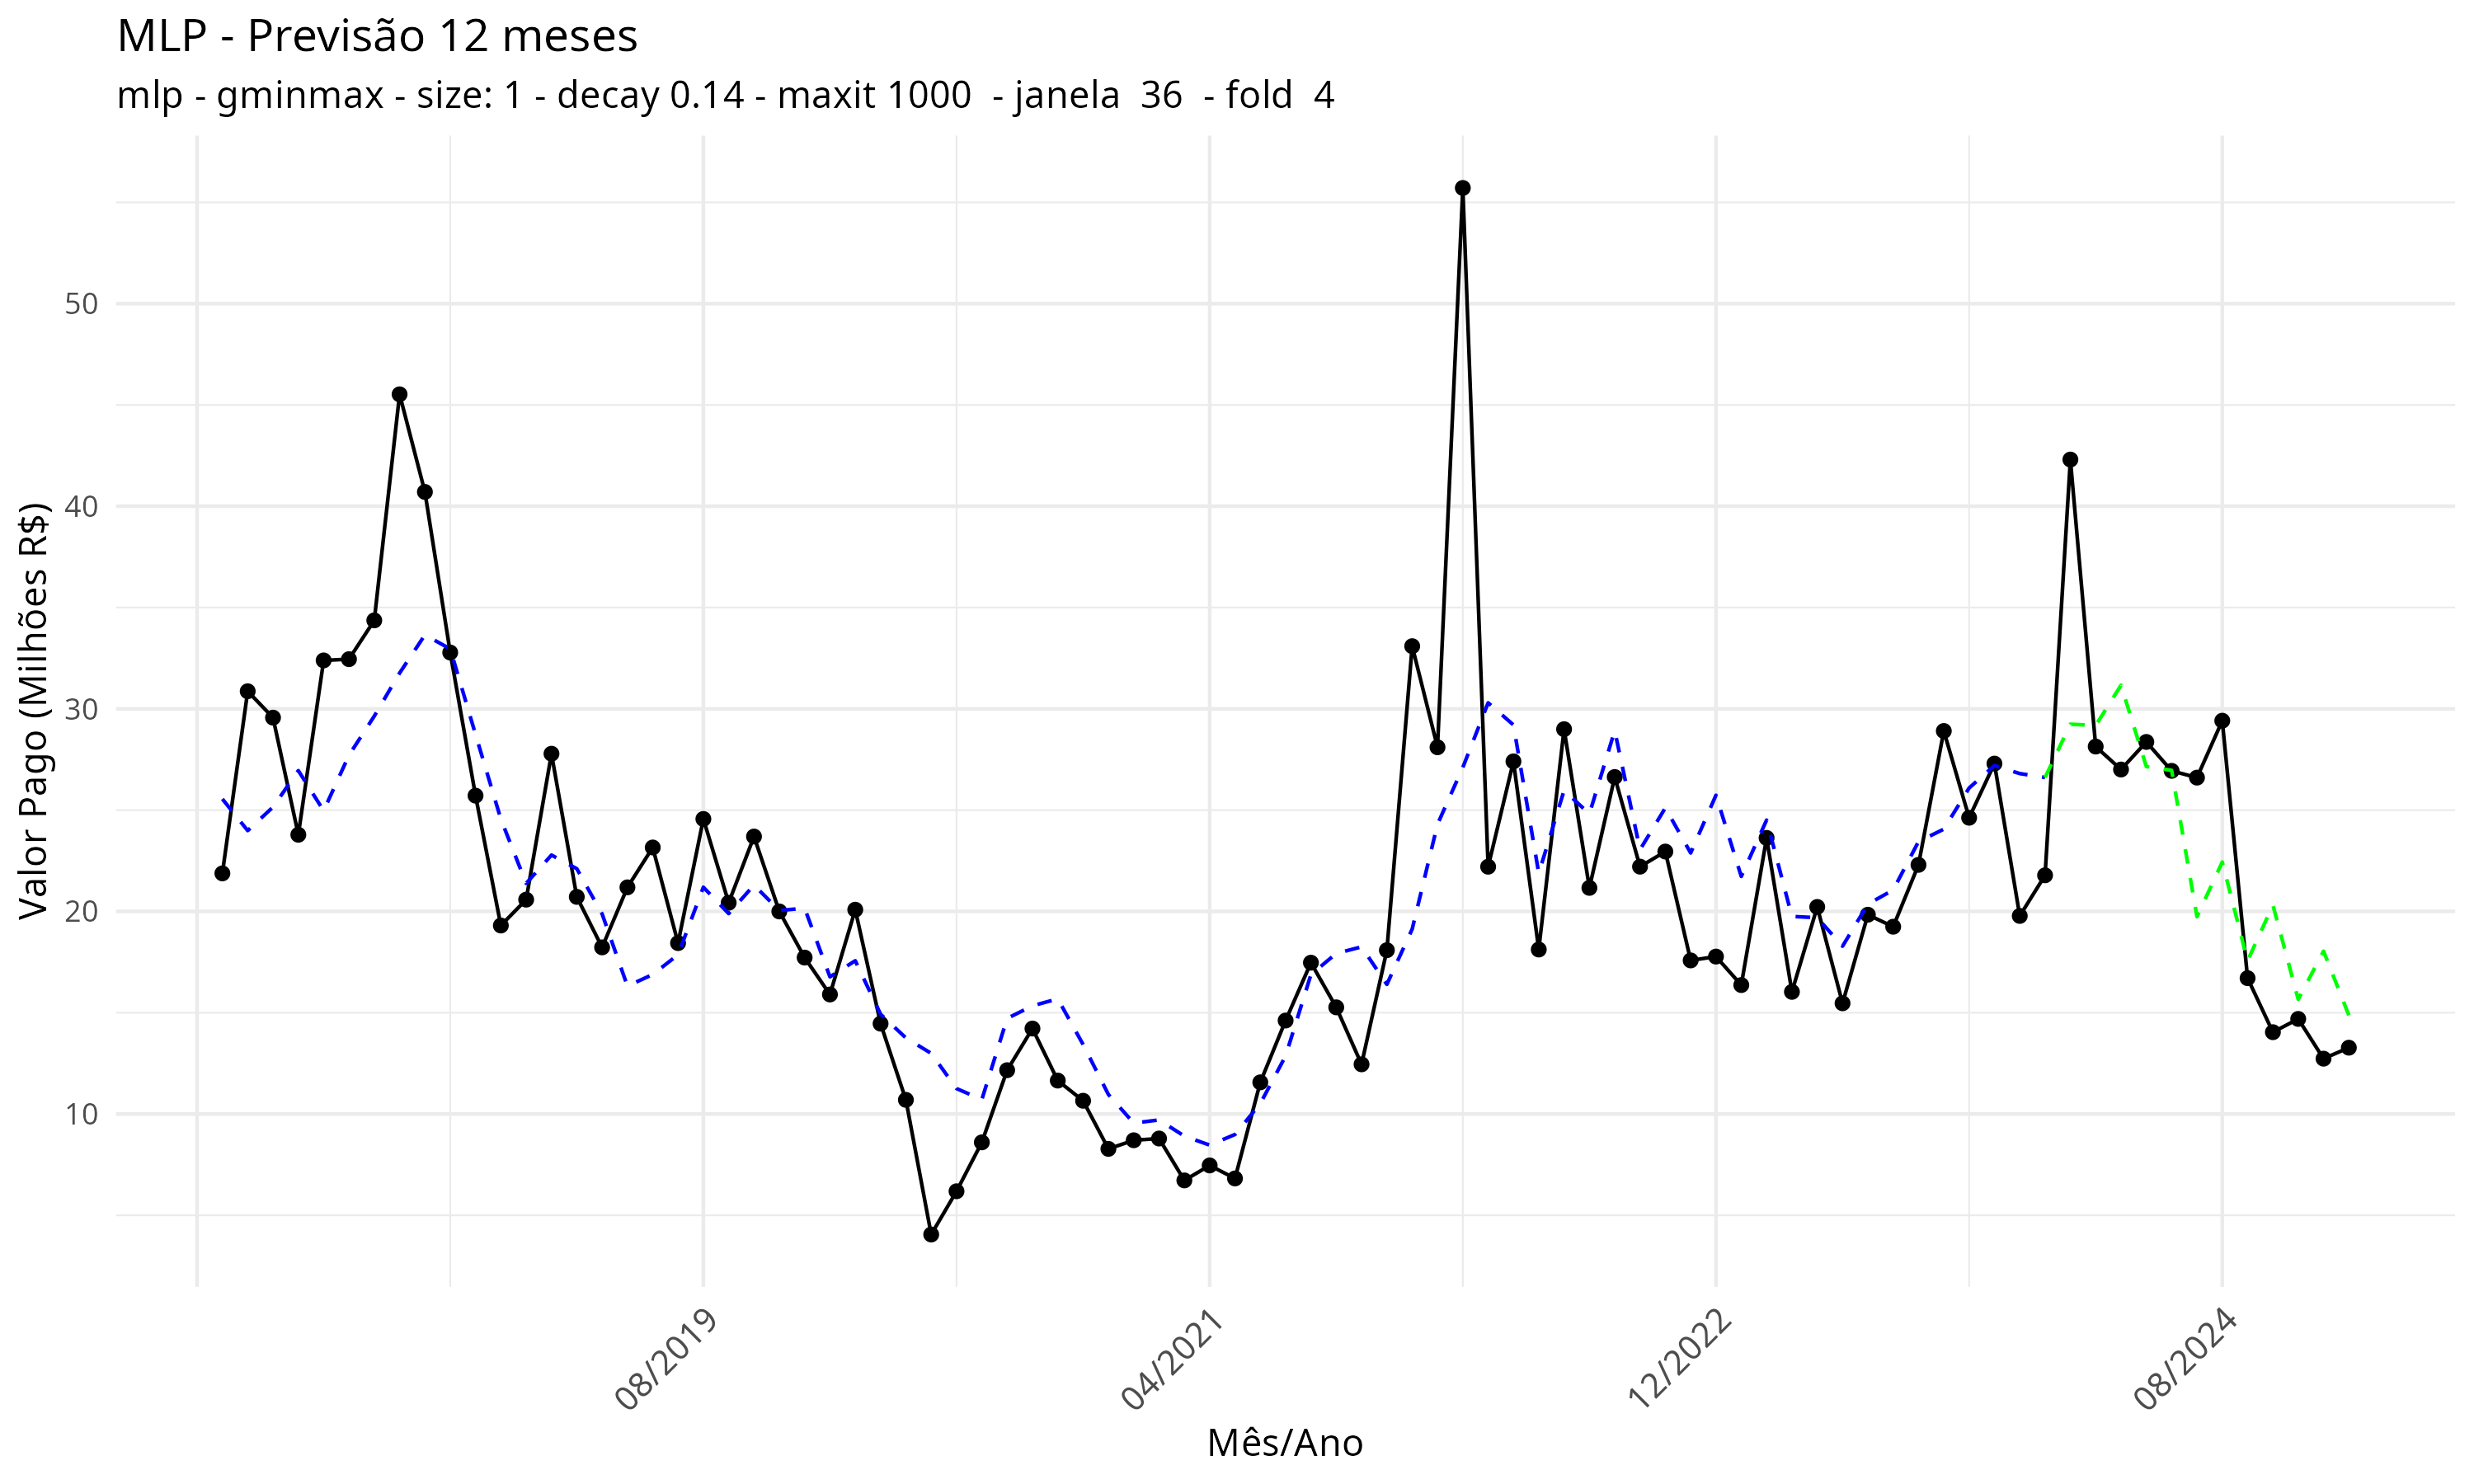
\includegraphics[width=0.8\textwidth]{figures/mlp-gminmax-s1-d014-m1000_janela-36_fold-4_plot.png}
	\caption{Previsão da receita no período de 12 meses com o modelo MLP - fold 4.}
	\label{fig:mlp12mesesfold4}
\end{figure}

\begin{figure}[!ht]
	\centering
	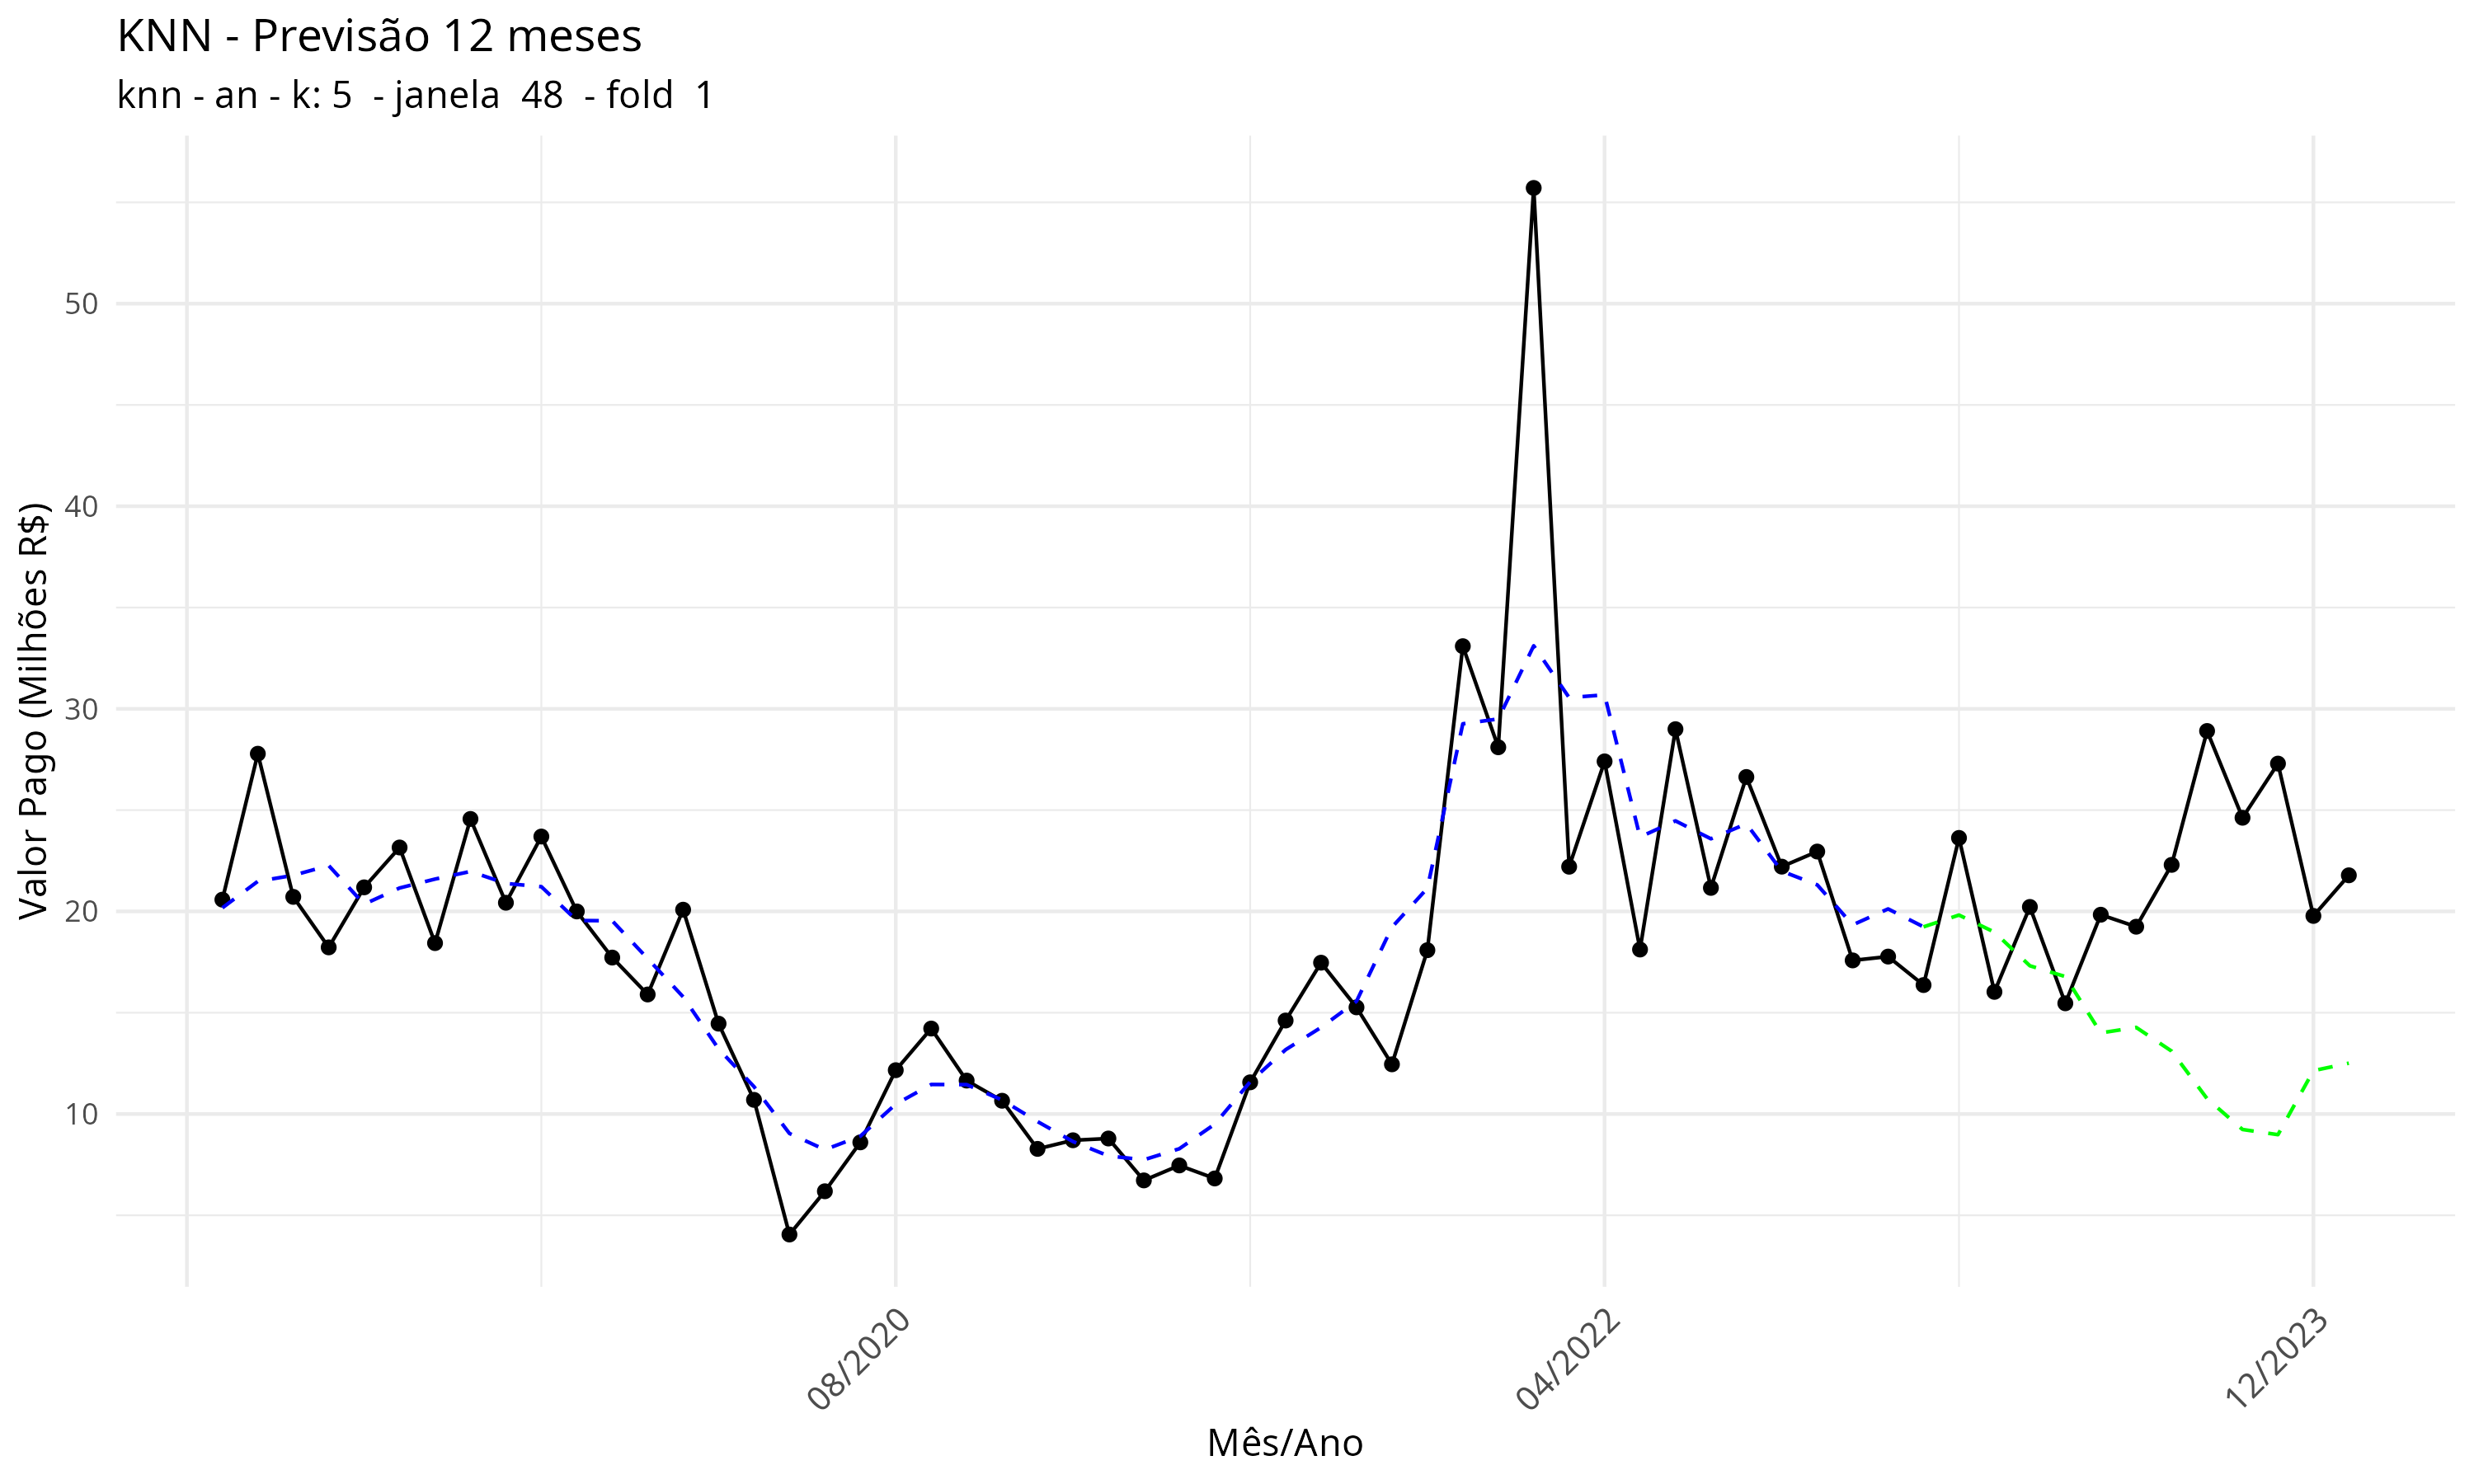
\includegraphics[width=0.8\textwidth]{figures/knn-k5_janela-48_fold-1_plot.png}
	\caption{Previsão da receita no período de 12 meses com o modelo KNN - fold 1.}
	\label{fig:knn12mesesfold1}
\end{figure}

\begin{figure}[!ht]
	\centering
	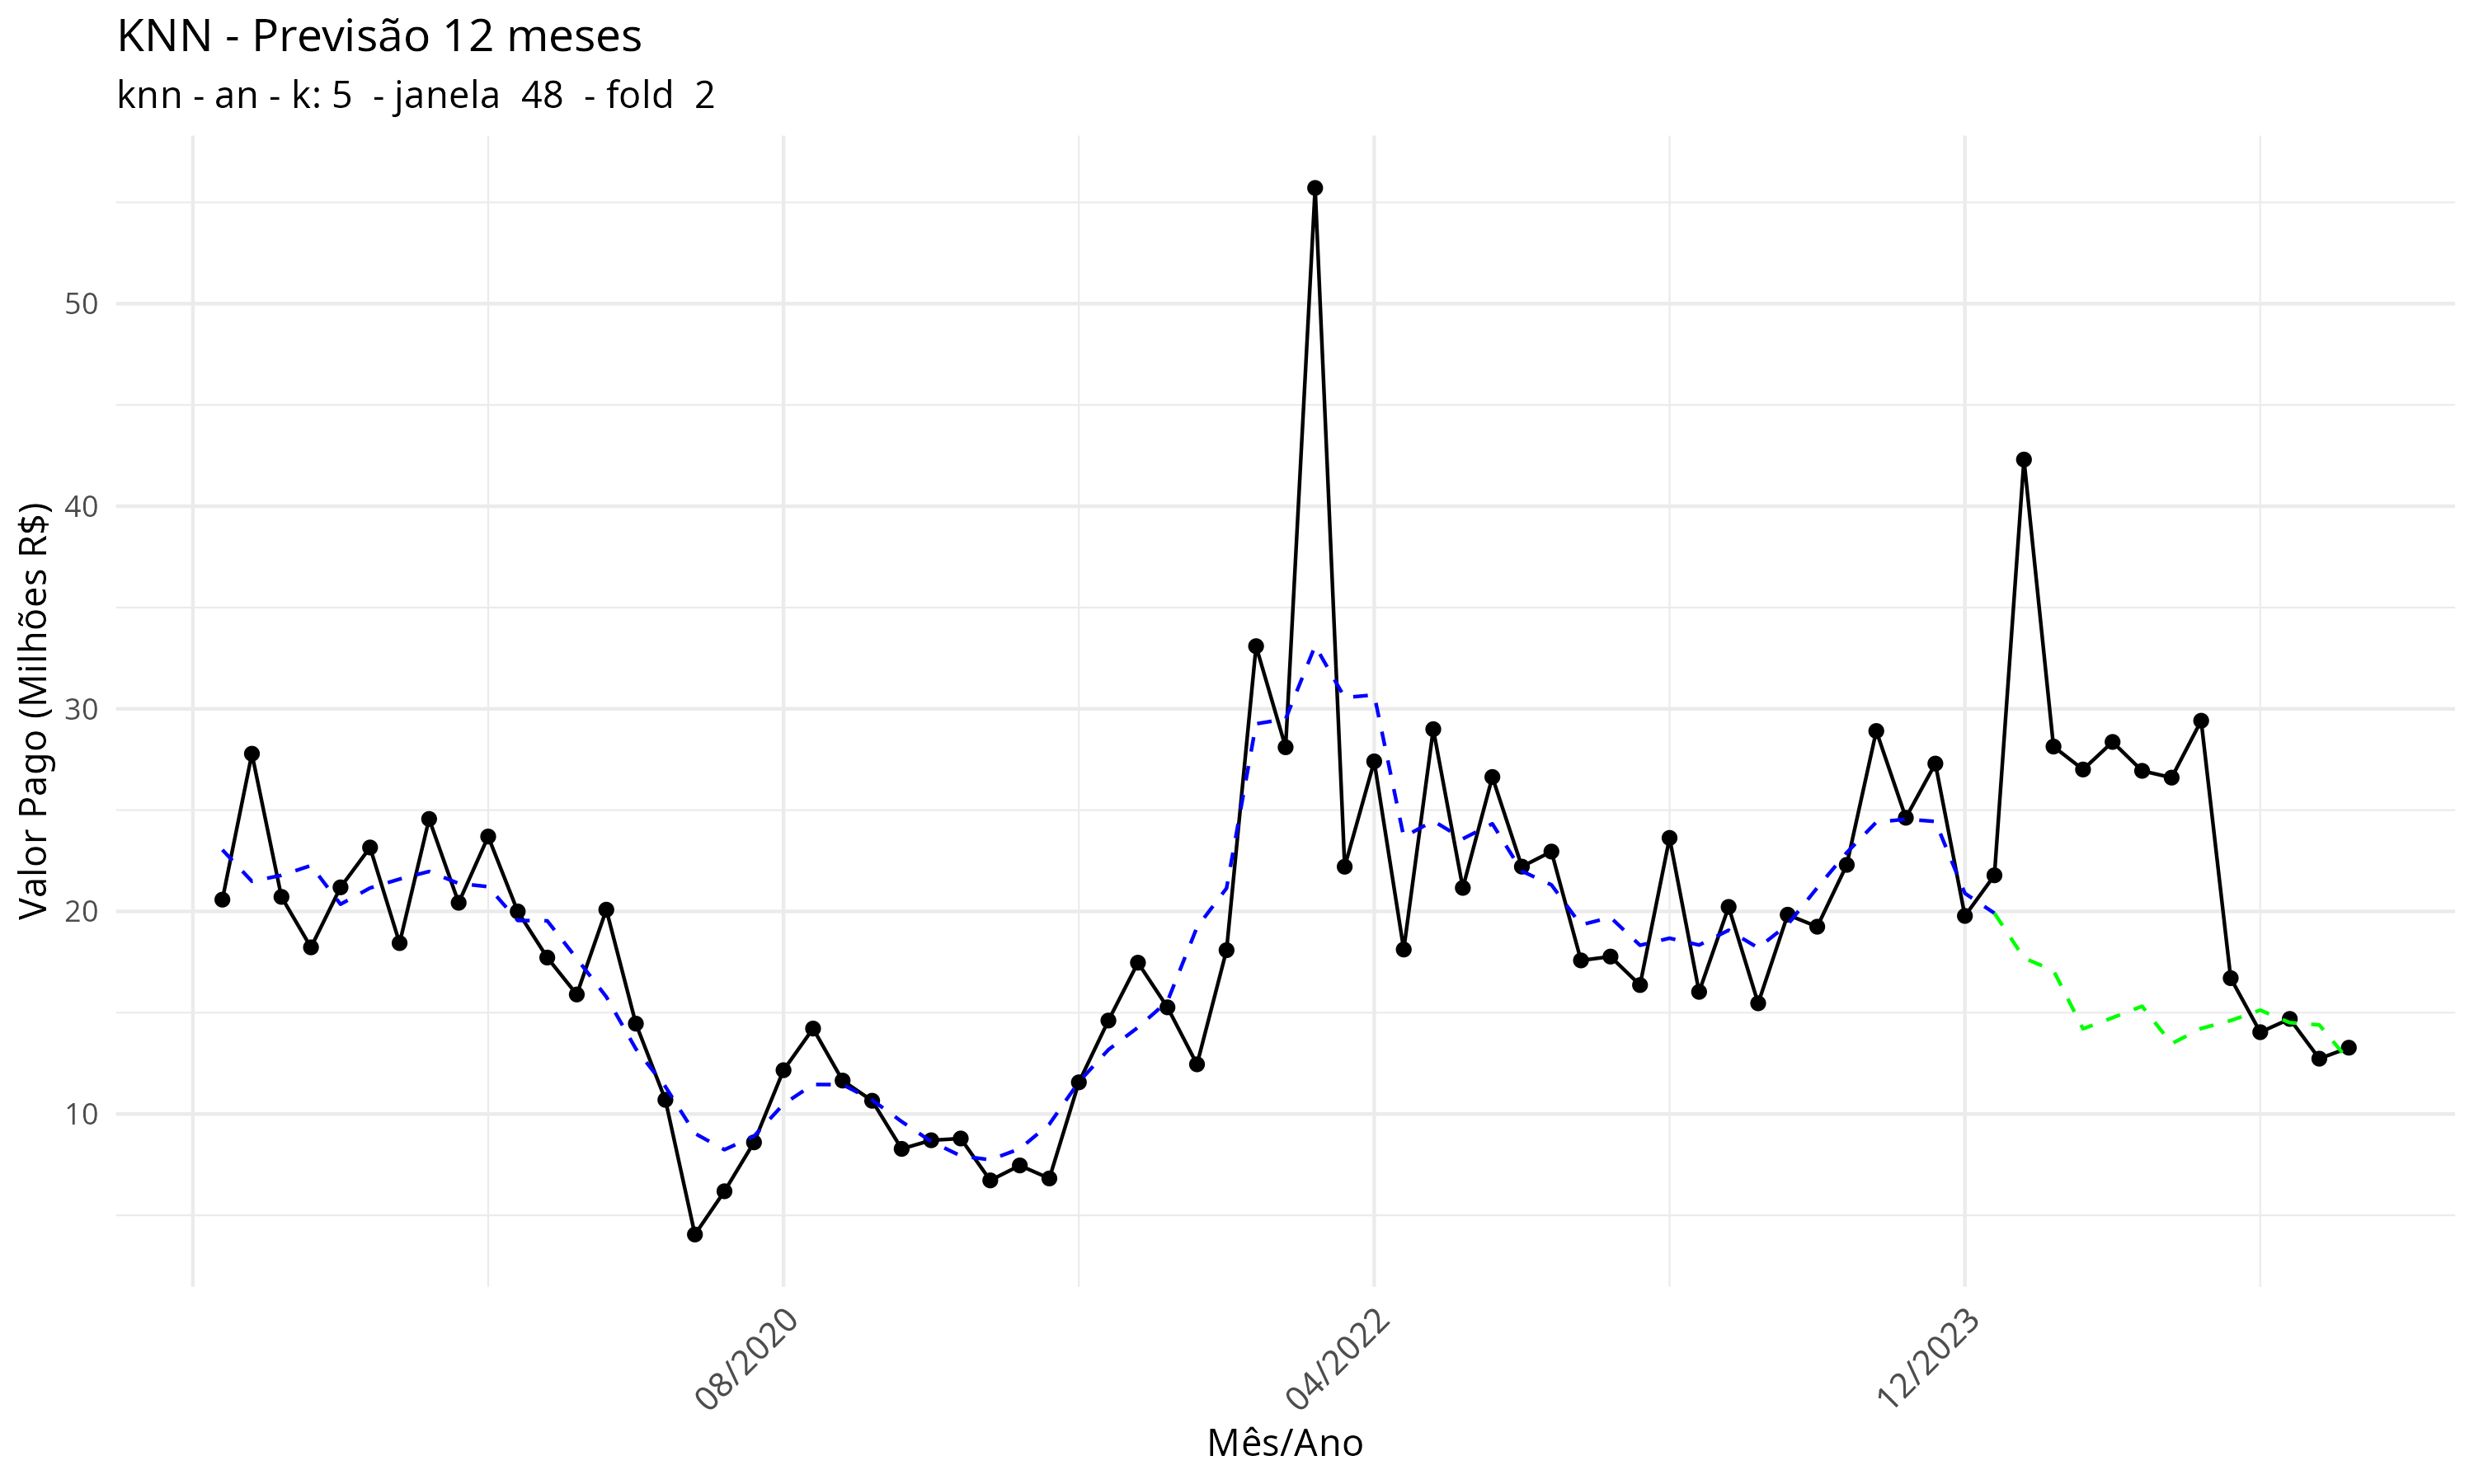
\includegraphics[width=0.8\textwidth]{figures/knn-k5_janela-48_fold-2_plot.png}
	\caption{Previsão da receita no período de 12 meses com o modelo KNN - fold 2.}
	\label{fig:knn12mesesfold2}
\end{figure}

\chapter{Conclusão}
\label{sec:conclusao}

Tendo em vista o propósito do trabalho de verificar a possibilidade de um modelo de aprendizado de máquina que seja capaz de prever o período de um ano da série de multas de trânsito, conclui-se que modelos de aprendizado de máquina é consideravelmente eficaz que o convencionalmente utilizado, baseado nos trabalhos relacionados a esse mesmo escopo. No que diz respeito à agregação temporal, esta técnica mostra sua relevância na redução de outliers da série temporal. Considerando o contexto, de acordo com \citeauthor{Rostami2013Demand} à medida que a série cresce, é possível que se tenha dados suficientes para reduzir esse horizonte de previsão, aumentando o desempenhos dos modelos. 

A série de multas de trânsito mostrou um comportamento capaz de ser previsto para certos modelos e configurações. Apesar da baixa quantidade de dados históricos, o MLP apresentou desempenho muito satisfatório ao obter $R^2$ com 60.26\% para a previsão de um ano. Dado esse resultado, conclui-se que modelos de aprendizado de máquina podem ser utilizados para prever receitas de multas de trânsito nesse período.

Este trabalho considerou a previsão da série temporal de multas de trânsito do período de janeiro de 2014 a dezembro de 2024. Não foi possível, portanto, apresentar os resultados junto ao ano de 2025. Acrescentar os dados históricos do ano de 2025 pode revelar detalhes importantes sobre os modelos apresentados. Sugere-se também que trabalhos futuros testem outros modelos de aprendizado de máquina, como os modelos aprendizado profundo.



\newcommand{\Extrachap}[1]{\chapter*{#1}\markboth{#1}{#1}
\addcontentsline{toc}{chapter}{#1}}

\Extrachap{Referências}

\renewcommand{\bibsection}{}
\renewcommand{\bibname}{}

\bibliography{references}
\bibliographystyle{apalike}
\label{bibfinalpage}

\label{lastpage}
\end{document}
